\documentclass[aps,prl,reprint,superscriptaddress,nofootinbib,floatfix]{revtex4-2}

\makeatletter
\def\bibdata@ext{notes}% keep the auto-generated REVTeX Notes file from being parsed as a .bib
\makeatother

\usepackage[T1]{fontenc}
\usepackage{amsmath,amssymb,amsthm,mathtools}
\usepackage{newtxtext,newtxmath}
\usepackage{microtype}
\usepackage{tikz}
\usetikzlibrary{arrows.meta,fit,positioning}
\definecolor{pptblue}{HTML}{316A91}
\definecolor{pptorange}{HTML}{BF793B}
\definecolor{pptpurple}{HTML}{74668B}
\definecolor{pptgreen}{HTML}{287D70}
\definecolor{pptink}{HTML}{253342}
\usepackage[colorlinks=true,allcolors=blue]{hyperref}

\allowdisplaybreaks

\newcommand{\M}{\mathrm{M}}
\newcommand{\I}{\mathrm{I}}
\newcommand{\C}{\mathbb C}
\newcommand{\id}{\operatorname{id}}
\newcommand{\Ad}{\operatorname{Ad}}
\newcommand{\Tr}{\operatorname{Tr}}
\newcommand{\PPT}{\operatorname{PPT}}
\newcommand{\EB}{\operatorname{EB}}
\newcommand{\CP}{\operatorname{CP}}
\newcommand{\SEP}{\operatorname{SEP}}
\newcommand{\SN}{\operatorname{SN}}
\newcommand{\Sym}{\operatorname{Sym}}
\newcommand{\supp}{\operatorname{supp}}
\newcommand{\vecop}{\operatorname{vec}}
\newcommand{\cB}{\mathcal B}
\newcommand{\cU}{\mathcal U}
\newcommand{\Tmap}{\mathsf T}

\newtheorem{theorem}{Theorem}
\newtheorem{lemma}[theorem]{Lemma}
\newtheorem{proposition}[theorem]{Proposition}
\newtheorem{corollary}[theorem]{Corollary}
\newcommand{\suppsection}[2]{%
 \refstepcounter{section}%
 \section*{\thesection.\ #1}%
 \label{sm:#2}}

\begin{document}

\title{A Qubit Forbids Entanglement Swapping between PPT Links}
\author{Ao-Xiang Liu}
\affiliation{School of Physical Sciences, University of Chinese Academy of Sciences, 1 Yanqihu East Rd, Beijing 101408, China}
\author{Cong-Feng Qiao}
\email[]{qiaocf@ucas.ac.cn}
\affiliation{School of Physical Sciences, University of Chinese Academy of Sciences, 1 Yanqihu East Rd, Beijing 101408, China}
\affiliation{ICTP-AP, University of Chinese Academy of Sciences, Beijing 100190, China}
\date{September 27, 2026}

\begin{abstract}
The positive partial transpose (PPT) squared conjecture posited that applying a completely positive and completely copositive map twice inevitably produces an entanglement-breaking map. We prove that two PPT maps compose to an entanglement-breaking map whenever the input, intermediate, or output system is a qubit, with the other dimensions arbitrary and independent. Translated to the state picture, we establish that the conditional state of the end systems is separable for every measurement outcome on the intermediate systems of two independent PPT states whenever any one of the four local systems is a qubit. Furthermore, the composition of any two composable PPT maps is shown to be 2-entanglement breaking, as is its adjoint, with each successive pair reducing the Schmidt number by at least one when acting locally on a bipartite state until separability is reached, even along a chain of varying dimensions. In particular, any sequence of $2(d-1)$ PPT maps on a $d$-dimensional system composes to an entanglement-breaking map.
\end{abstract}

\maketitle

\textit{Introduction.---}
Quantum channels are composed whenever a noisy physical process is applied repeatedly or elementary links are connected within a quantum network. Entanglement-breaking maps destroy entanglement with every reference system and therefore limit quantum communication~\cite{Horodecki2003}. Positive partial transpose (PPT) maps form a larger class whose Choi operators may still contain bound entanglement~\cite{Horodecki1998}. Whether this entanglement survives composition matters both for repeated noise and for connecting PPT links in a quantum repeater~\cite{Briegel1998,Bauml2015}.

The PPT squared conjecture proposed that applying any PPT map twice produces an entanglement-breaking map, without assuming trace preservation. Christandl, M\"uller-Hermes, and Wolf proved that this is equivalent to the two-map formulation for two possibly different PPT maps with compatible dimensions~\cite{Christandl2019}. Through the Choi--Jamio\l{}kowski correspondence, composition is related to entanglement swapping~\cite{Zukowski1993}. A maximally entangled projection on the intermediate systems of two Choi states yields an operator proportional to the Choi operator of the composed map~\cite{Singh2022,An2026}. Local filtering extends this correspondence to arbitrary selective measurements~\cite{An2026}, connecting composition to the ability of two independent PPT links to distribute entanglement between remote parties.

The two-map problem for qubit maps follows from the low-dimensional separability criterion~\cite{Horodecki1996} and was subsequently settled for qutrits by Christandl \textit{et al.} and by Chen, Yang, and Tang~\cite{Christandl2019,Chen2019}. Further results cover Gaussian channels and Choi-type maps~\cite{Christandl2019,Singh2022}. More recently, two qutrit completely positive (CP) maps were shown to compose to an entanglement-breaking map when one Choi operator is one-copy undistillable and the other has Schmidt number at most two, in either order~\cite{An2026}. Henry proved that an intermediate qubit suffices even for arbitrary input and output dimensions~\cite{Henry2026}.

Recent counterexamples rule out the unrestricted conjecture. Two PPT maps on a ten-dimensional system can have a composition that is not entanglement breaking, and a trace-preserving PPT channel in dimension twenty-one can have a non-entanglement-breaking square~\cite{OpenAI2026}. These examples leave open which dimensions force two-step entanglement breaking and how many PPT maps always suffice.

At an endpoint, a qubit presents a different difficulty. The adjacent Choi operator can be PPT entangled when its other subsystem has dimension at least four~\cite{Horodecki1997}, leaving the low-dimensional separability criterion insufficient to settle the composition. The case of a qubit input was already identified in 2019 as a missing premise for a uniform bound on the number of PPT compositions needed to destroy entanglement~\cite{Christandl2019}. Its resolution therefore constrains repeated composition even in the absence of a qubit.

For repeated applications of a single map, the entanglement-breaking index counts the uses needed to destroy entanglement with every reference system~\cite{Lami2015}. Asymptotic convergence to entanglement-breaking maps was first established for unital or trace-preserving PPT maps~\cite{Kennedy2018}. Finite indices were subsequently proved under unitality or full-rank assumptions on Perron eigenmatrices~\cite{Rahaman2018,Hanson2020}, and then for every PPT linear map~\cite{Park2026}. For unital channels, spectral structure also characterizes eventual entanglement breaking and its equivalence to eventual PPT~\cite{Bhat2026}. Finiteness for each map does not by itself give a common bound depending only on dimension, the question posed by Park~\cite{Park2026}.

In this work, we prove that two PPT maps compose to an entanglement-breaking map whenever the input, intermediate, or output system is a qubit, with the other dimensions arbitrary and independent. For the endpoint cases, we represent the adjacent Choi operator through a positive auxiliary qutrit operator invariant under partial transposition. Each pure term in its decomposition has qutrit support in a two-dimensional subspace with a real orthonormal basis. Symmetrizing the positive maps then makes their restrictions decomposable, establishing the required nonnegative pairing. An independent Pauli argument treats the intermediate case. In the state formulation, two independent PPT links yield a separable state of the end systems for every measurement outcome whenever any one of the four local systems is a qubit, even when the intermediate systems differ in dimension.

The endpoint result also supplies the premise needed for the iteration argument of Ref.~\cite{Christandl2019}. In arbitrary dimensions, the composition of any two compatible PPT maps and its adjoint are 2-entanglement breaking. Each successive pair then reduces the Schmidt number by at least one when acting locally on a bipartite state until separability is reached, even along chains of changing dimensions. This gives a uniform entanglement-breaking index bound linear in dimension.


%%%%%%=========================================================================================

\textit{Main result.---}Let $\M_d$ denote the algebra of complex $d\times d$ matrices. For a linear map $\Phi:\M_p\to\M_q$, its unnormalized Choi operator is defined as
\begin{equation}
 J_\Phi=\sum_{i,j=0}^{p-1}E_{ij}\otimes\Phi(E_{ij})\ ,
\label{eq:choi}
\end{equation}
where $E_{ij}=|i\rangle\langle j|$ denote the standard matrix units and $\Tmap_d(Z)=Z^{\mathsf T}$ is transposition in a fixed orthonormal basis. The partial transpose $\Gamma$ acts on the second factor. A map $\Phi$ is PPT if $J_\Phi\succeq0$ and $J_\Phi^\Gamma\succeq0$, and entanglement breaking (EB) if $J_\Phi$ belongs to the cone $\SEP$ of separable positive operators~\cite{Choi1975,Horodecki2003}. Throughout, trace preservation and unitality are not assumed, and no rank restrictions are imposed.

\begin{theorem}
\label{thm:anywhere}
Let
\begin{equation}
 \Phi_1:\M_{d_0}\longrightarrow\M_{d_1},\qquad
 \Phi_2:\M_{d_1}\longrightarrow\M_{d_2}
\label{eq:pair}
\end{equation}
be PPT maps. If $2\in\{d_0,d_1,d_2\}$, then the composition $\Phi_2\circ\Phi_1$ is entanglement breaking, with the remaining two dimensions arbitrary and independent.
\end{theorem}

We establish the case $d_2=2$ directly and deduce $d_0=2$ by Hilbert--Schmidt adjunction. An independent Pauli argument establishes the intermediate case $d_1=2$.

\begin{figure}[!t]
\centering
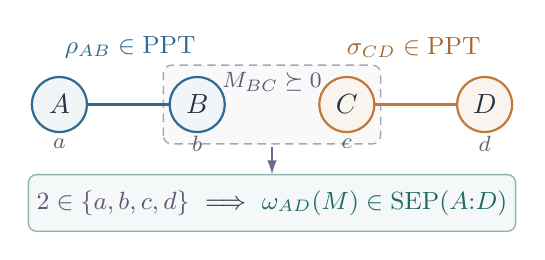
\begin{tikzpicture}[
  text=pptink,
  site/.style={circle,line width=0.8pt,
    minimum size=7mm,inner sep=0pt,font=\fontsize{10}{11}\selectfont},
  dim/.style={font=\fontsize{8}{9}\selectfont,text=pptink!75},
  state/.style={font=\fontsize{9}{10}\selectfont},
  result/.style={rounded corners=3pt,draw=pptgreen!55,
    fill=pptgreen!5,line width=0.5pt,minimum width=5.35cm,
    minimum height=7.2mm,inner sep=3pt,
    font=\fontsize{9}{10}\selectfont}
]
\node[state,text=pptblue] at (0.90,0.72) {$\rho_{AB}\in\PPT$};
\node[state,text=pptorange!85!black] at (4.50,0.72)
  {$\sigma_{CD}\in\PPT$};
\path[rounded corners=3pt,fill=pptpurple!4,draw=pptpurple!60,
  line width=0.5pt,densely dashed]
  (1.32,-0.50) rectangle (4.08,0.50);
\draw[pptblue,line width=0.9pt] (0,0)--(1.75,0);
\draw[pptorange,line width=0.9pt] (3.65,0)--(5.40,0);
\node[site,draw=pptblue,fill=pptblue!7] (A) at (0,0) {$A$};
\node[site,draw=pptblue,fill=pptblue!7] (B) at (1.75,0) {$B$};
\node[site,draw=pptorange,fill=pptorange!8] (C) at (3.65,0) {$C$};
\node[site,draw=pptorange,fill=pptorange!8] (D) at (5.40,0) {$D$};
\node[dim] at (0,-0.50) {$a$};
\node[dim] at (1.75,-0.50) {$b$};
\node[dim] at (3.65,-0.50) {$c$};
\node[dim] at (5.40,-0.50) {$d$};
\node[font=\fontsize{8}{9}\selectfont,text=pptpurple!85!black]
  at (2.70,0.29) {$M_{BC}\succeq0$};
\draw[-{Latex[length=1.8mm,width=1.2mm]},pptpurple,line width=0.65pt]
  (2.70,-0.54)--(2.70,-0.89);
\node[result] at (2.70,-1.25)
  {$\textcolor{pptpurple!85!black}{2\in\{a,b,c,d\}}
    \ \Longrightarrow\
    \textcolor{pptgreen!85!black}{\omega_{AD}(M)\in\SEP(A{:}D)}$};
\end{tikzpicture}
\caption{One-shot entanglement swapping across two independent PPT states with arbitrary local dimensions $a,b,c,d$. For any positive measurement operator $M=M_{BC}\succeq0$ on the intermediate systems, the unnormalized conditional state $\omega_{AD}(M)$ on the end systems is separable whenever $2\in\{a,b,c,d\}$.}
\label{fig:swapping}
\end{figure}

%%%%%=======================================================================================================================
\textit{Composition with a two-dimensional output system.---}When the output algebra is $\M_2$, the PPT Choi operator of the second map may itself be entangled~\cite{Horodecki1997}. Separability of the composed Choi operator can instead be tested through its pairing with the Choi operators of all positive maps. This gives the following equivalent bilinear positivity statement. Here, $\PPT(n,d)$ denotes the cone of positive operators on $\C^n\otimes\C^d$ whose partial transpose on the second factor is positive, while $\I_n$ and $\id_n$ denote the identity matrix and identity map on $\M_n$, respectively.

\begin{lemma}
\label{thm:bilinear}
For all $n,d\geq1$, every positive map $T:\M_2\to\M_d$, every $X\in\PPT(n,d)$, and every $R\in\PPT(n,2)$,
\begin{equation}
 \Tr\!\left[X(\id_n\otimes T)(R)\right]\geq0\ .
\label{eq:bilinear}
\end{equation}
\end{lemma}

Equation~\eqref{eq:bilinear} requires nonnegativity of the pairing with every PPT operator $X$, even though $(\id_n\otimes T)(R)$ can fail to be positive. We establish this pairing by representing $R$ as the image of a positive operator $Q$ invariant under partial transposition on an auxiliary qutrit factor. The auxiliary dimension separates the two Hermitian components of the qubit off-diagonal block while retaining this symmetry. We then decompose $Q$ into pure components whose qutrit supports lie in two-dimensional complex subspaces with real orthonormal bases. Symmetrizing the positive map on the auxiliary factor leaves its action on $Q$ unchanged and makes its restrictions to these subspaces decomposable.

\begin{lemma}
\label{lem:realplanes}
Every positive operator $Q\in\M_n\otimes\M_3$ satisfying $Q^{\Gamma_{\mathrm{qutrit}}}=Q$ admits a decomposition
\begin{align}
 Q=\sum_{s=1}^{r}|\psi_s\rangle\langle\psi_s|\ ,
 \qquad (\I_n\otimes a_s^{\mathsf T})\psi_s=0\ ,
\label{eq:realplanes}
\end{align}
where $r=\operatorname{rank}Q$ and $a_s\in\mathbb R^3\setminus\{0\}$. If $Q=0$, the decomposition is empty.
\end{lemma}

The additional content beyond the known Schmidt-number bound~\cite{Huber2018} is the real orthonormal basis for the subspace containing each qutrit support. A bound of two on the Schmidt number alone does not ensure this property. In the proof (detailed in Ref.~\cite{Supplement}), partial-transpose invariance makes the cross products of Gram blocks Hermitian. A real linear combination of these blocks achieves full column rank on the marginal support, and a Hermitian extension mapping one block to another gives the decomposition through the spectral theorem.

For any $R\in\PPT(n,2)$, we construct such an operator $Q$ satisfying
\begin{align}
 (\id_n\otimes\Ad_V)(Q)=R,\qquad
 V=\begin{pmatrix}1&-i&0\\0&0&1\end{pmatrix}\ ,
\label{eq:recovery}
\end{align}
where $\Ad_L(Z)=LZL^*$. In qubit-first block notation, $R=\left(\begin{smallmatrix}A&C\\C^*&B\end{smallmatrix}\right)$ with $C=X_R+iY_R$ and $X_R=X_R^*, Y_R=Y_R^*$. The construction uses
\begin{equation}
 \begin{aligned}
 G&=B^+,& \Delta&=A-X_RGX_R-Y_RGY_R,\\[-1mm]
 W&=Y_RGX_R-X_RGY_R,& \Xi&=X_RGY_R+Y_RGX_R\ .
 \end{aligned}
\label{eq:auxiliaryblocks}
\end{equation}
Here, $B^+$ and $P_B$ denote the Moore--Penrose pseudoinverse and support projector of $B$, respectively. Generalized Schur complements~\cite{Albert1969} give $X_R=P_BX_RP_B$, $Y_R=P_BY_RP_B$, and $\Delta\pm iW\succeq0$. The auxiliary operator in qutrit-first order is
\begin{equation}
 \widetilde Q=
 \begin{pmatrix}
  X_RGX_R+\Delta/2&-\Xi/2&X_R\\
  -\Xi/2&Y_RGY_R+\Delta/2&-Y_R\\
  X_R&-Y_R&B
 \end{pmatrix}\ ,
\label{eq:auxiliaryQ}
\end{equation}
with $\widetilde Q\in\M_3\otimes\M_n$. The tensor flip $F_{3,n}(u\otimes v)=v\otimes u$ gives $Q=F_{3,n}\widetilde QF_{3,n}^*\in\M_n\otimes\M_3$. Direct multiplication confirms Eq.~\eqref{eq:recovery}, while the block symmetry of $\widetilde Q$ gives $Q^{\Gamma_{\mathrm{qutrit}}}=Q$. Subtracting the Gram operator with block column $(X_R,-Y_R,B)^{\mathsf T}$ and weight $G$ leaves a residual whose nonzero spectral blocks are $(\Delta\mp iW)/2$. Thus $Q\succeq0$, and Lemma~\ref{lem:realplanes} applies. The explicit splitting and treatment of singular supports appear in Ref.~\cite{Supplement}.

The real basis preserves transposition under restriction. For a real isometry $U:\C^2\to\C^3$, one has $\Tmap_3\circ\Ad_U=\Ad_U\circ\Tmap_2$, an identity not guaranteed for a general complex isometry. If a positive map $\Lambda:\M_3\to\M_k$ satisfies $\Lambda=\Lambda\circ\Sym$ with $\Sym(Z)=(Z+Z^{\mathsf T})/2$, its restriction consequently satisfies $\Lambda\circ\Ad_U=(\Lambda\circ\Ad_U)\circ\Tmap_2$. The restricted map is decomposable by the separability of positive $2\otimes k$ operators invariant under qubit partial transposition~\cite{Kraus2000} and the duality between the PPT cone and decomposable witnesses~\cite{Stormer1982,Skowronek2009}. According to Lemma~\ref{lem:realplanes}, each component vector can be written as $\psi_s=\sum_i|i\rangle\otimes U_sC_s|i\rangle$, where $U_s:\C^2\to\C^3$ is a real isometry and $C_s:\C^n\to\C^2$. Its image under the partial map is
\begin{align}
 (\id_n\otimes\Lambda)(|\psi_s\rangle\langle\psi_s|)
 &=J_{(\Lambda\circ\Ad_{U_s})\circ\Ad_{C_s}}\ .
\label{eq:componentchoi}
\end{align}
Because precomposition with a CP map preserves decomposability, each resulting operator is decomposable and thus pairs nonnegatively with any PPT operator, yielding
\begin{equation}
 \Tr\!\left[P(\id_n\otimes\Lambda)(Q)\right]\geq0
 \qquad\text{for all }P\in\PPT(n,k)\ .
\label{eq:nonnegativepairing}
\end{equation}

For the given positive map $T:\M_2\to\M_d$, we can now take
\begin{align}
 \Lambda=T\circ\Ad_V\circ\Sym:\M_3\to\M_d\ .
\label{eq:Lambda}
\end{align}
Each factor is positive, so $\Lambda$ is positive. Idempotence of $\Sym$ gives $\Lambda=\Lambda\circ\Sym$. Moreover, $Q^{\Gamma_{\mathrm{qutrit}}}=Q$ implies $(\id_n\otimes\Sym)(Q)=Q$, so symmetrization leaves the recovered operator unchanged. Denoting the pairing in Eq.~\eqref{eq:bilinear} by $\cB_T(X,R)$, Eqs.~\eqref{eq:recovery} and \eqref{eq:nonnegativepairing} give
\begin{align}
 \cB_T(X,R)
 &=\Tr\!\left[X(\id_n\otimes\Lambda)(Q)\right]\geq0\ .
\label{eq:directpairing}
\end{align}
This proves Lemma~\ref{thm:bilinear} without any rank assumption on $T$.

Lemma~\ref{thm:bilinear} resolves the case of a two-dimensional output system. For any PPT maps $\Phi:\M_d\to\M_n$ and $\Psi:\M_n\to\M_2$, the Hilbert--Schmidt adjoint $\Phi^*$ is also PPT, giving $X=J_{\Phi^*}\in\PPT(n,d)$ and $R=J_\Psi\in\PPT(n,2)$. A direct contraction over matrix units shows that
\begin{align}
 \cB_T(J_{\Phi^*},J_\Psi)
 &=\Tr_{\rm HS}(T\circ\Psi\circ\Phi)
 =\Tr\!\left[J_{T^*}J_{\Psi\circ\Phi}\right]\ ,
\label{eq:choipairing}
\end{align}
where $\Tr_{\rm HS}S=\sum_{i,j}\Tr[E_{ji}S(E_{ij})]$. As $T:\M_2\to\M_d$ sweeps over all positive maps, $J_{T^*}$ exhausts the cone of block-positive operators. Lemma~\ref{thm:bilinear} ensures that Eq.~\eqref{eq:choipairing} is nonnegative for every such operator. Duality between the cones of block-positive and separable operators~\cite{Horodecki1996} then implies that $J_{\Psi\circ\Phi}$ is separable, and hence $\Psi\circ\Phi$ is entanglement breaking. Applying the identical argument to the adjoint PPT pair $(\Psi^*,\Phi^*)$ resolves the case of a two-dimensional input system.

%%%%%%%=========================================================================================================================

\textit{Two-dimensional intermediate system.---}Recently, Henry established the case of a two-dimensional intermediate system by analyzing normalized $2\times2$ Choi blocks via operator interpolation~\cite{Henry2026}. Here, we present an independent, self-contained proof based on the qubit spin-flip symmetry and an explicit separability identity for matrix contractions.

\begin{lemma}
\label{lem:rowgram}
Let $X_j\in\M_a$ and $Y_j\in\M_c$ ($j=1,\ldots,r$) be Hermitian operators. If
\begin{equation}
 \sum_jX_j^2\preceq\I_a,\qquad
 \sum_jY_j^2\preceq\I_c\ ,
\label{eq:rowbounds}
\end{equation}
then the bipartite operator $\I_a\otimes\I_c+\sum_jX_j\otimes Y_j$ is separable across $\C^a{:}\C^c$.
\end{lemma}

Indeed, defining the positive and negative parts $X_j^\pm=(|X_j|\pm X_j)/2$ with $|X_j|=\sqrt{X_j^2}$ (and similarly for $Y_j$), the operator bounds in Eq.~\eqref{eq:rowbounds} ensure that the deficits $D_X=\I_a-\sum_jX_j^2$ and $D_Y=\I_c-\sum_jY_j^2$ are positive semidefinite. A direct algebraic expansion gives
\begin{align}
 \I\otimes\I+\sum_jX_j\otimes Y_j
 &=2\sum_j(X_j^+\otimes Y_j^++X_j^-\otimes Y_j^-)
 \nonumber\\*
 &\quad+\tfrac12 D_X\otimes\I+\tfrac12\I\otimes D_Y
 \nonumber\\*
 &\quad+\tfrac12\sum_j
 (|X_j|\otimes\I-\I\otimes|Y_j|)^2\ .
\label{eq:rowidentity}
\end{align}
For each $j$, a product of eigenbases of $|X_j|$ and $|Y_j|$ makes $(|X_j|\otimes\I-\I\otimes|Y_j|)^2$ diagonal with nonnegative entries and therefore separable. All remaining terms are positive product operators, which proves the lemma.

To establish the case $d_1=2$, let $\Phi_1:\M_{d_0}\to\M_2$ and $\Phi_2:\M_2\to\M_{d_2}$ be PPT maps. We set $\Psi=\Phi_1^*$ and $\Theta=\Phi_2$, and whiten them on their respective output supports to obtain unital PPT maps $\widehat\Psi$ and $\widehat\Theta$. Evaluating these maps on the three Pauli matrices $\sigma_j$ ($j=1,2,3$), we define the Hermitian operators $X_j=\widehat\Psi(\sigma_j)$ and $Y_j=\widehat\Theta(\sigma_j)$. Complete positivity, complete copositivity, and the qubit spin-flip symmetry $(\Tmap_2\circ\Ad_{\sigma_y})(\sigma_j)=-\sigma_j$ imply
\begin{equation}
 -\I\preceq\sum_{j=1}^3\sigma_j^{\mathsf T}\otimes X_j\preceq\I\ .
\label{eq:spinflip}
\end{equation}
Squaring this operator inequality and evaluating the normalized partial trace over the qubit factor yields $\sum_jX_j^2\preceq\I$, with an identical bound $\sum_jY_j^2\preceq\I$ holding for $Y_j$. Consequently, the composite Choi operator
\begin{equation}
 J_{\widehat\Theta\circ\widehat\Psi^*}
 =\tfrac12\left(\I\otimes\I+
   \sum_{j=1}^3X_j^{\mathsf T}\otimes Y_j\right)
\label{eq:middlechoi}
\end{equation}
is separable by Lemma~\ref{lem:rowgram}. Reversing the whitening transformation via local completely positive congruences preserves separability, thereby establishing the result for $d_1=2$ (the technical treatment of singular output supports is detailed in Ref.~\cite{Supplement}). Combined with the input and output cases established above, this completes the proof of Theorem~\ref{thm:anywhere}.

%%%%==============================================================================================

\textit{Entanglement swapping and consequences for composition.---}Theorem~\ref{thm:anywhere} gives an operational statement for the two independent PPT states in Fig.~\ref{fig:swapping}. With one copy of each state and the relay quantum output discarded, a measurement effect $0\preceq M_{BC}\preceq\I_{BC}$ prepares the unnormalized conditional state
\begin{equation}
\omega_{AD}(M)=\Tr_{BC}\!\left[(\rho_{AB}\otimes\sigma_{CD})
 (\I_A\otimes M_{BC}\otimes\I_D)\right]\ .
\label{eq:swapping}
\end{equation}
The same expression applies to any positive $M_{BC}$, since rescaling it to a physical effect does not change separability.

\begin{corollary}
\label{cor:swapping}
Let $\dim A=a$, $\dim B=b$, $\dim C=c$, and $\dim D=d$. If $\rho_{AB}\in\PPT(A{:}B)$, $\sigma_{CD}\in\PPT(C{:}D)$, and $2\in\{a,b,c,d\}$, then
\begin{equation}
 \omega_{AD}(M)\in\SEP(A{:}D)\qquad\text{for every }M_{BC}\succeq0\ .
\label{eq:selective}
\end{equation}
\end{corollary}

Following the local-filtering argument of Ref.~\cite{An2026}, a vector $|\eta\rangle\in B\otimes C$ admits two representations using rectangular matrices even when the intermediate dimensions differ,
\begin{equation}
 |\eta\rangle=(L_B\otimes\I_C)|\Omega_c\rangle
 =(\I_B\otimes L_C)|\Omega_b\rangle\ ,
\label{eq:tworepresentations}
\end{equation}
where $B',C'$ are copies of $B,C$, $L_B:C'\to B$, $L_C=L_B^{\mathsf T}:B'\to C$, and $|\Omega_q\rangle=\sum_{j=0}^{q-1}|j\rangle\otimes|j\rangle$. Absorbing these rectangular filters into the PPT states maps the contraction to a standard maximally entangled projection on $C'{:}C$ or $B{:}B'$, covering a qubit at $\{A,C,D\}$ or $B$, respectively. Spectral decomposition of $M_{BC}$ then establishes Corollary~\ref{cor:swapping} (singular filters and local CP operations are treated in Ref.~\cite{Supplement}).

The Schmidt number $\SN(Z)$ of a nonzero positive bipartite operator is the least possible maximal Schmidt rank among its pure-state decompositions. If $M_{BC}\neq0$ and $\SN(M_{BC})\leq2$, decomposing $M_{BC}$ into pure terms reduces each contribution to a maximally entangled qubit projection after local filtering. The intermediate case of Theorem~\ref{thm:anywhere} then makes $\omega_{AD}(M)$ separable for arbitrary local dimensions. This uses Henry's composition result~\cite{Henry2026} and the same principle as Park's three-factor result~\cite{Park2026}. A zero effect gives the zero operator, which is separable.

A CP map $K:\M_p\to\M_q$ is \emph{2-entanglement breaking} (2-EB) if $(\id_2\otimes K)(Z)$ is separable for every $Z\succeq0$ in $\M_2\otimes\M_p$~\cite{Christandl2019}, or equivalently, if $K\circ E$ is EB for every CP map $E:\M_2\to\M_p$~\cite{Devendra2023}.

\begin{corollary}
\label{cor:twoeb}
Let $\Phi_1:\M_{d_0}\to\M_{d_1}$ and $\Phi_2:\M_{d_1}\to\M_{d_2}$ be PPT maps. Then both $H=\Phi_2\circ\Phi_1$ and its adjoint $H^*=\Phi_1^*\circ\Phi_2^*$ are 2-EB.
\end{corollary}

For any CP map $E_0:\M_2\to\M_{d_0}$, the map $\Phi_1\circ E_0$ is PPT. The $d_0=2$ case of Theorem~\ref{thm:anywhere} therefore makes $H\circ E_0$ EB. Applying the same argument to the adjoint pair $(\Phi_2^*,\Phi_1^*)$ proves the claim for $H^*$. This separate application is needed because the class of 2-EB maps is not generally closed under adjoints~\cite{Devendra2023}.

\begin{corollary}
\label{cor:index}
For any $2\ell$ compatible PPT maps $\Phi_j:\M_{d_{j-1}}\to\M_{d_j}$ ($\ell\geq1$), let $H_{2\ell}=\Phi_{2\ell}\circ\cdots\circ\Phi_1$. Every positive bipartite input $Z$ satisfies
\begin{align}
 \SN\!\left[(\id\otimes H_{2\ell})(Z)\right]
 \leq\max\{\SN(Z)-\ell,1\}\ ,
\label{eq:schmidtdecay}
\end{align}
whenever the output is nonzero. Zero outputs are separable.
\end{corollary}

The composition of each adjacent pair is 2-EB by Corollary~\ref{cor:twoeb}. For any pure input component of Schmidt rank $s\geq2$, compressing the reference system to dimension $s$ allows the result of Ref.~\cite{Christandl2019} to bound the output Schmidt number by $s-1$ whenever the output dimension is at least $s$. A smaller output dimension already gives this bound, while separable inputs remain separable under local CP maps. Iterating over $\ell$ pairs proves Eq.~\eqref{eq:schmidtdecay}.

For a chain $H_N=\Phi_N\circ\cdots\circ\Phi_1$ with input and output dimensions $d_0$ and $d_N$, applying the Schmidt decay to the Choi input and to the adjoint chain yields
\begin{align}
 N\geq2\bigl(\min\{d_0,d_N\}-1\bigr)
 \quad\Longrightarrow\quad H_N\text{ is EB}\ ,
\label{eq:rectangularindex}
\end{align}
for arbitrary intermediate dimensions. For PPT maps $T:\M_d\to\M_d$ ($d\geq2$), the entanglement-breaking index $n_{\rm EB}(T)=\min\{n\geq1:T^n\text{ is EB}\}$ therefore satisfies
\begin{align}
 \sup_T n_{\rm EB}(T)\leq2(d-1)\ .
\label{eq:indexbound}
\end{align}
The implication from the statement for a qubit input to 2-EB squares and the bound $2(d-1)$ was already established conditionally in Ref.~\cite{Christandl2019}. Theorem~\ref{thm:anywhere} supplies the missing premise, making the bound unconditional and answering Park's question on a bound depending only on dimension~\cite{Park2026}. Park's dimension-independent three- and five-step bounds require additional restrictions on the maps~\cite{Park2026}. Our bound applies to all PPT maps, but is not optimal for qutrits, where two steps suffice~\cite{Christandl2019,Chen2019}.

%%%%%%==============================================================================================================

\textit{Conclusions.---}
The endpoint result closes the qubit case of PPT composition even when the adjacent Choi operator is entangled. Its proof depends on more than a bound on Schmidt number. The real orthonormal bases in the auxiliary decomposition preserve transposition under restriction, allowing the relevant positive maps to be treated through decomposability. Together with the intermediate case, this shows that a qubit in any of the four original local systems prevents two independent PPT links from producing entanglement between the endpoints in a single swapping operation, for every measurement outcome and at every rank. Neither link is required to be separable.

The high-dimensional counterexamples~\cite{OpenAI2026} show that PPT entanglement can survive the composition of two PPT maps when no system is a qubit. By Corollary~\ref{cor:twoeb}, these non-entanglement-breaking compositions and their adjoints are nevertheless 2-entanglement breaking. They destroy entanglement with every qubit reference but can retain it with a larger reference. Thus 2-entanglement breaking is strictly weaker than entanglement breaking even within the class of compositions of two PPT maps.

The Schmidt-number iteration controls this surviving entanglement under further composition and gives the uniform index bound $\sup_T n_{\rm EB}(T)\leq2(d-1)$. The failure of the unrestricted two-map conjecture is therefore compatible with a bound linear in dimension on the number of PPT maps needed to destroy all entanglement. Determining the optimal bound, and which dimensions beyond a qubit still force two-step entanglement breaking, remain open questions. Extending the endpoint argument requires control of positive maps on larger subspaces or of operators lacking the partial-transpose symmetry used here.

\textit{Acknowledgments.---}
This work was supported in part by the National Natural Science Foundation of
China (NSFC) under Grants No.~12475087 and No.~12235008.


% References are embedded below. Edit the bibitem entries directly.
%apsrev4-2.bst 2019-01-14 (MD) hand-edited version of apsrev4-1.bst
%Control: key (0)
%Control: author (72) initials jnrlst
%Control: editor formatted (1) identically to author
%Control: production of article title (-1) disabled
%Control: page (0) single
%Control: year (1) truncated
%Control: production of eprint (0) enabled
\begin{thebibliography}{27}%
\makeatletter
\providecommand \@ifxundefined [1]{%
 \@ifx{#1\undefined}
}%
\providecommand \@ifnum [1]{%
 \ifnum #1\expandafter \@firstoftwo
 \else \expandafter \@secondoftwo
 \fi
}%
\providecommand \@ifx [1]{%
 \ifx #1\expandafter \@firstoftwo
 \else \expandafter \@secondoftwo
 \fi
}%
\providecommand \natexlab [1]{#1}%
\providecommand \enquote  [1]{``#1''}%
\providecommand \bibnamefont  [1]{#1}%
\providecommand \bibfnamefont [1]{#1}%
\providecommand \citenamefont [1]{#1}%
\providecommand \href@noop [0]{\@secondoftwo}%
\providecommand \href [0]{\begingroup \@sanitize@url \@href}%
\providecommand \@href[1]{\@@startlink{#1}\@@href}%
\providecommand \@@href[1]{\endgroup#1\@@endlink}%
\providecommand \@sanitize@url [0]{\catcode `\\12\catcode `\$12\catcode
  `\&12\catcode `\#12\catcode `\^12\catcode `\_12\catcode `\%12\relax}%
\providecommand \@@startlink[1]{}%
\providecommand \@@endlink[0]{}%
\providecommand \url  [0]{\begingroup\@sanitize@url \@url }%
\providecommand \@url [1]{\endgroup\@href {#1}{\urlprefix }}%
\providecommand \urlprefix  [0]{URL }%
\providecommand \Eprint [0]{\href }%
\providecommand \doibase [0]{https://doi.org/}%
\providecommand \selectlanguage [0]{\@gobble}%
\providecommand \bibinfo  [0]{\@secondoftwo}%
\providecommand \bibfield  [0]{\@secondoftwo}%
\providecommand \translation [1]{[#1]}%
\providecommand \BibitemOpen [0]{}%
\providecommand \bibitemStop [0]{}%
\providecommand \bibitemNoStop [0]{.\EOS\space}%
\providecommand \EOS [0]{\spacefactor3000\relax}%
\providecommand \BibitemShut  [1]{\csname bibitem#1\endcsname}%
\let\auto@bib@innerbib\@empty
%</preamble>
\bibitem [{\citenamefont {Horodecki}\ \emph {et~al.}(2003)\citenamefont
  {Horodecki}, \citenamefont {Shor},\ and\ \citenamefont
  {Ruskai}}]{Horodecki2003}%
  \BibitemOpen
  \bibfield  {author} {\bibinfo {author} {\bibfnamefont {M.}~\bibnamefont
  {Horodecki}}, \bibinfo {author} {\bibfnamefont {P.~W.}\ \bibnamefont
  {Shor}},\ and\ \bibinfo {author} {\bibfnamefont {M.~B.}\ \bibnamefont
  {Ruskai}},\ }\bibfield {title} {\bibinfo {title} {Entanglement Breaking Channels}, }\href {https://doi.org/10.1142/S0129055X03001709} {\bibfield
  {journal} {\bibinfo  {journal} {Rev. Math. Phys.}\ }\textbf
  {\bibinfo {volume} {15}},\ \bibinfo {pages} {629} (\bibinfo {year}
  {2003})}\BibitemShut {NoStop}%
\bibitem [{\citenamefont {Horodecki}\ \emph {et~al.}(1998)\citenamefont
  {Horodecki}, \citenamefont {Horodecki},\ and\ \citenamefont
  {Horodecki}}]{Horodecki1998}%
  \BibitemOpen
  \bibfield  {author} {\bibinfo {author} {\bibfnamefont {M.}~\bibnamefont
  {Horodecki}}, \bibinfo {author} {\bibfnamefont {P.}~\bibnamefont
  {Horodecki}},\ and\ \bibinfo {author} {\bibfnamefont {R.}~\bibnamefont
  {Horodecki}},\ }\bibfield {title} {\bibinfo {title} {Mixed-State Entanglement and Distillation: Is There a ``Bound'' Entanglement in Nature?}, }\href {https://doi.org/10.1103/PhysRevLett.80.5239}
  {\bibfield  {journal} {\bibinfo  {journal} {Phys. Rev. Lett.}\
  }\textbf {\bibinfo {volume} {80}},\ \bibinfo {pages} {5239} (\bibinfo {year}
  {1998})}\BibitemShut {NoStop}%
\bibitem [{\citenamefont {Briegel}\ \emph {et~al.}(1998)\citenamefont
  {Briegel}, \citenamefont {D\"ur}, \citenamefont {Cirac},\ and\ \citenamefont
  {Zoller}}]{Briegel1998}%
  \BibitemOpen
  \bibfield  {author} {\bibinfo {author} {\bibfnamefont {H.-J.}\ \bibnamefont
  {Briegel}}, \bibinfo {author} {\bibfnamefont {W.}~\bibnamefont {D\"ur}},
  \bibinfo {author} {\bibfnamefont {J.~I.}\ \bibnamefont {Cirac}},\ and\
  \bibinfo {author} {\bibfnamefont {P.}~\bibnamefont {Zoller}},\ }\bibfield {title} {\bibinfo {title} {Quantum Repeaters: The Role of Imperfect Local Operations in Quantum Communication}, }\href
  {https://doi.org/10.1103/PhysRevLett.81.5932} {\bibfield  {journal} {\bibinfo
   {journal} {Phys. Rev. Lett.}\ }\textbf {\bibinfo {volume} {81}},\
  \bibinfo {pages} {5932} (\bibinfo {year} {1998})}\BibitemShut {NoStop}%
\bibitem [{\citenamefont {B\"auml}\ \emph {et~al.}(2015)\citenamefont
  {B\"auml}, \citenamefont {Christandl}, \citenamefont {Horodecki},\ and\
  \citenamefont {Winter}}]{Bauml2015}%
  \BibitemOpen
  \bibfield  {author} {\bibinfo {author} {\bibfnamefont {S.}~\bibnamefont
  {B\"auml}}, \bibinfo {author} {\bibfnamefont {M.}~\bibnamefont {Christandl}},
  \bibinfo {author} {\bibfnamefont {K.}~\bibnamefont {Horodecki}},\ and\
  \bibinfo {author} {\bibfnamefont {A.}~\bibnamefont {Winter}},\ }\bibfield {title} {\bibinfo {title} {Limitations on Quantum Key Repeaters}, }\href
  {https://doi.org/10.1038/ncomms7908} {\bibfield  {journal} {\bibinfo
  {journal} {Nat. Commun.}\ }\textbf {\bibinfo {volume} {6}},\
  \bibinfo {pages} {6908} (\bibinfo {year} {2015})}\BibitemShut {NoStop}%
\bibitem [{\citenamefont {Christandl}\ \emph {et~al.}(2019)\citenamefont
  {Christandl}, \citenamefont {M\"uller-Hermes},\ and\ \citenamefont
  {Wolf}}]{Christandl2019}%
  \BibitemOpen
  \bibfield  {author} {\bibinfo {author} {\bibfnamefont {M.}~\bibnamefont
  {Christandl}}, \bibinfo {author} {\bibfnamefont {A.}~\bibnamefont
  {M\"uller-Hermes}},\ and\ \bibinfo {author} {\bibfnamefont {M.~M.}\
  \bibnamefont {Wolf}},\ }\bibfield {title} {\bibinfo {title} {When Do Composed Maps Become Entanglement Breaking?}, }\href {https://doi.org/10.1007/s00023-019-00774-7}
  {\bibfield  {journal} {\bibinfo  {journal} {Ann. Henri Poincar{\'e}}\
  }\textbf {\bibinfo {volume} {20}},\ \bibinfo {pages} {2295} (\bibinfo {year}
  {2019})}\BibitemShut {NoStop}%
\bibitem [{\citenamefont {{\.{Z}}ukowski}\ \emph {et~al.}(1993)\citenamefont
  {{\.{Z}}ukowski}, \citenamefont {Zeilinger}, \citenamefont {Horne},\ and\
  \citenamefont {Ekert}}]{Zukowski1993}%
  \BibitemOpen
  \bibfield  {author} {\bibinfo {author} {\bibfnamefont {M.}~\bibnamefont
  {{\.{Z}}ukowski}}, \bibinfo {author} {\bibfnamefont {A.}~\bibnamefont
  {Zeilinger}}, \bibinfo {author} {\bibfnamefont {M.~A.}\ \bibnamefont
  {Horne}},\ and\ \bibinfo {author} {\bibfnamefont {A.~K.}\ \bibnamefont
  {Ekert}},\ }\bibfield {title} {\bibinfo {title} {``Event-Ready-Detectors'' Bell Experiment via Entanglement Swapping}, }\href {https://doi.org/10.1103/PhysRevLett.71.4287} {\bibfield
  {journal} {\bibinfo  {journal} {Phys. Rev. Lett.}\ }\textbf {\bibinfo
  {volume} {71}},\ \bibinfo {pages} {4287} (\bibinfo {year}
  {1993})}\BibitemShut {NoStop}%
\bibitem [{\citenamefont {Singh}\ and\ \citenamefont
  {Nechita}(2022)}]{Singh2022}%
  \BibitemOpen
  \bibfield  {author} {\bibinfo {author} {\bibfnamefont {S.}~\bibnamefont
  {Singh}}\ and\ \bibinfo {author} {\bibfnamefont {I.}~\bibnamefont
  {Nechita}},\ }\bibfield {title} {\bibinfo {title} {The {PPT}$^2$ Conjecture Holds for All Choi-Type Maps}, }\href {https://doi.org/10.1007/s00023-022-01166-0} {\bibfield
  {journal} {\bibinfo  {journal} {Ann. Henri Poincar{\'e}}\ }\textbf
  {\bibinfo {volume} {23}},\ \bibinfo {pages} {3311} (\bibinfo {year}
  {2022})}\BibitemShut {NoStop}%
\bibitem [{\citenamefont {An}\ and\ \citenamefont {Lee}(2026)}]{An2026}%
  \BibitemOpen
  \bibfield  {author} {\bibinfo {author} {\bibfnamefont {J.}~\bibnamefont
  {An}}\ and\ \bibinfo {author} {\bibfnamefont {S.}~\bibnamefont {Lee}},\
  }\bibfield {title} {\bibinfo {title} {Beyond the Positive Partial Transpose Squared Conjecture: The Qutrit Case}, }\Eprint {https://arxiv.org/abs/2607.15947} {arXiv:2607.15947}
  (\bibinfo {year} {2026})
  \BibitemShut {NoStop}%
\bibitem [{\citenamefont {Horodecki}\ \emph {et~al.}(1996)\citenamefont
  {Horodecki}, \citenamefont {Horodecki},\ and\ \citenamefont
  {Horodecki}}]{Horodecki1996}%
  \BibitemOpen
  \bibfield  {author} {\bibinfo {author} {\bibfnamefont {M.}~\bibnamefont
  {Horodecki}}, \bibinfo {author} {\bibfnamefont {P.}~\bibnamefont
  {Horodecki}},\ and\ \bibinfo {author} {\bibfnamefont {R.}~\bibnamefont
  {Horodecki}},\ }\bibfield {title} {\bibinfo {title} {Separability of Mixed States: Necessary and Sufficient Conditions}, }\href {https://doi.org/10.1016/S0375-9601(96)00706-2}
  {\bibfield  {journal} {\bibinfo  {journal} {Phys. Lett. A}\ }\textbf
  {\bibinfo {volume} {223}},\ \bibinfo {pages} {1} (\bibinfo {year}
  {1996})}\BibitemShut {NoStop}%
\bibitem [{\citenamefont {Chen}\ \emph {et~al.}(2019)\citenamefont {Chen},
  \citenamefont {Yang},\ and\ \citenamefont {Tang}}]{Chen2019}%
  \BibitemOpen
  \bibfield  {author} {\bibinfo {author} {\bibfnamefont {L.}~\bibnamefont
  {Chen}}, \bibinfo {author} {\bibfnamefont {Y.}~\bibnamefont {Yang}},\ and\
  \bibinfo {author} {\bibfnamefont {W.-S.}\ \bibnamefont {Tang}},\ }\bibfield {title} {\bibinfo {title} {Positive-Partial-Transpose Square Conjecture for $n=3$}, }\href
  {https://doi.org/10.1103/PhysRevA.99.012337} {\bibfield  {journal} {\bibinfo
  {journal} {Phys. Rev. A}\ }\textbf {\bibinfo {volume} {99}},\ \bibinfo
  {pages} {012337} (\bibinfo {year} {2019})}\BibitemShut {NoStop}%
\bibitem [{\citenamefont {Henry}(2026)}]{Henry2026}%
  \BibitemOpen
  \bibfield  {author} {\bibinfo {author} {\bibfnamefont {K.}~\bibnamefont
  {Henry}},\ }\bibfield {title} {\bibinfo {title} {{PPT} Composition Through a Qubit Is Entanglement Breaking}, }{Zenodo} (\bibinfo {year} {2026}), \href
  {https://doi.org/10.5281/zenodo.21866485}
  {doi:10.5281/zenodo.21866485}\BibitemShut {NoStop}%
\bibitem [{\citenamefont {OpenAI}(2026)}]{OpenAI2026}%
  \BibitemOpen
  \bibfield {author} {\bibinfo {author} {\bibnamefont {OpenAI}},\ }
  \bibfield {title} {\bibinfo {title} {Entanglement with Zero Distillable Secret Key in Local Dimension Ten},\ }
  \href {https://github.com/openai/math/blob/main/preprints/Entanglement-with-zero-distillable-secret-key-in-local-dimension-ten-September-27-2026/paper.pdf}
  {OpenAI Math Release preprint} (\bibinfo {year} {2026})\BibitemShut {NoStop}%
\bibitem [{\citenamefont {Horodecki}(1997)}]{Horodecki1997}%
  \BibitemOpen
  \bibfield  {author} {\bibinfo {author} {\bibfnamefont {P.}~\bibnamefont
  {Horodecki}},\ }\bibfield {title} {\bibinfo {title} {Separability Criterion and Inseparable Mixed States with Positive Partial Transposition}, }\href {https://doi.org/10.1016/S0375-9601(97)00416-7}
  {\bibfield  {journal} {\bibinfo  {journal} {Phys. Lett. A}\ }\textbf
  {\bibinfo {volume} {232}},\ \bibinfo {pages} {333} (\bibinfo {year}
  {1997})}\BibitemShut {NoStop}%
\bibitem [{\citenamefont {Lami}\ and\ \citenamefont
  {Giovannetti}(2015)}]{Lami2015}%
  \BibitemOpen
  \bibfield  {author} {\bibinfo {author} {\bibfnamefont {L.}~\bibnamefont
  {Lami}}\ and\ \bibinfo {author} {\bibfnamefont {V.}~\bibnamefont
  {Giovannetti}},\ }\bibfield {title} {\bibinfo {title} {Entanglement-Breaking Indices}, }\href {https://doi.org/10.1063/1.4931482} {\bibfield
  {journal} {\bibinfo  {journal} {J. Math. Phys.}\ }\textbf
  {\bibinfo {volume} {56}},\ \bibinfo {pages} {092201} (\bibinfo {year}
  {2015})}.\BibitemShut {Stop}%
\bibitem [{\citenamefont {Kennedy}\ \emph {et~al.}(2018)\citenamefont
  {Kennedy}, \citenamefont {Manor},\ and\ \citenamefont
  {Paulsen}}]{Kennedy2018}%
  \BibitemOpen
  \bibfield  {author} {\bibinfo {author} {\bibfnamefont {M.}~\bibnamefont
  {Kennedy}}, \bibinfo {author} {\bibfnamefont {N.~A.}\ \bibnamefont {Manor}},\
  and\ \bibinfo {author} {\bibfnamefont {V.~I.}\ \bibnamefont {Paulsen}},\
  }\bibfield {title} {\bibinfo {title} {Compositions of {PPT} Maps}, }\href {https://doi.org/10.26421/QIC18.5-6-4} {\bibfield  {journal} {\bibinfo
   {journal} {Quantum Inf. Comput.}\ }\textbf {\bibinfo {volume}
  {18}},\ \bibinfo {pages} {472} (\bibinfo {year} {2018})}\BibitemShut
  {NoStop}%
\bibitem [{\citenamefont {Rahaman}\ \emph {et~al.}(2018)\citenamefont
  {Rahaman}, \citenamefont {Jaques},\ and\ \citenamefont
  {Paulsen}}]{Rahaman2018}%
  \BibitemOpen
  \bibfield  {author} {\bibinfo {author} {\bibfnamefont {M.}~\bibnamefont
  {Rahaman}}, \bibinfo {author} {\bibfnamefont {S.}~\bibnamefont {Jaques}},\
  and\ \bibinfo {author} {\bibfnamefont {V.~I.}\ \bibnamefont {Paulsen}},\
  }\bibfield {title} {\bibinfo {title} {Eventually Entanglement Breaking Maps}, }\href {https://doi.org/10.1063/1.5024385} {\bibfield  {journal} {\bibinfo
  {journal} {J. Math. Phys.}\ }\textbf {\bibinfo {volume}
  {59}},\ \bibinfo {pages} {062201} (\bibinfo {year} {2018})}\BibitemShut
  {NoStop}%
\bibitem [{\citenamefont {Hanson}\ \emph {et~al.}(2020)\citenamefont {Hanson},
  \citenamefont {Rouz{\'e}},\ and\ \citenamefont {Stilck~Fran{\c
  c}a}}]{Hanson2020}%
  \BibitemOpen
  \bibfield  {author} {\bibinfo {author} {\bibfnamefont {E.~P.}\ \bibnamefont
  {Hanson}}, \bibinfo {author} {\bibfnamefont {C.}~\bibnamefont {Rouz{\'e}}},\
  and\ \bibinfo {author} {\bibfnamefont {D.}~\bibnamefont {Stilck~Fran{\c
  c}a}},\ }\bibfield {title} {\bibinfo {title} {Eventually Entanglement Breaking Markovian Dynamics: Structure and Characteristic Times}, }\href {https://doi.org/10.1007/s00023-020-00906-4} {\bibfield
  {journal} {\bibinfo  {journal} {Ann. Henri Poincar{\'e}}\ }\textbf
  {\bibinfo {volume} {21}},\ \bibinfo {pages} {1517} (\bibinfo {year}
  {2020})}\BibitemShut {NoStop}%
\bibitem [{\citenamefont {Park}(2026)}]{Park2026}%
  \BibitemOpen
  \bibfield  {author} {\bibinfo {author} {\bibfnamefont {S.-J.}\ \bibnamefont
  {Park}},\ }\bibfield {title} {\bibinfo {title} {Every {PPT} Channel Has Finite Entanglement-Breaking Index}, }\Eprint {https://arxiv.org/abs/2608.13551} {arXiv:2608.13551}
  (\bibinfo {year} {2026})
  \BibitemShut {NoStop}%
\bibitem [{\citenamefont {Bhat}\ \emph {et~al.}(2026)\citenamefont {Bhat},
  \citenamefont {Dey},\ and\ \citenamefont {Saha}}]{Bhat2026}%
  \BibitemOpen
  \bibfield  {author} {\bibinfo {author} {\bibfnamefont {B.~V.~R.}\
  \bibnamefont {Bhat}}, \bibinfo {author} {\bibfnamefont {P.}~\bibnamefont
  {Dey}},\ and\ \bibinfo {author} {\bibfnamefont {B.}~\bibnamefont {Saha}},\
  }\bibfield {title} {\bibinfo {title} {A Complete Characterization of Eventually Entanglement Breaking Unital Quantum Channels}, }\Eprint {https://arxiv.org/abs/2609.24168}
  {arXiv:2609.24168} (\bibinfo {year} {2026})\BibitemShut {NoStop}%
\bibitem [{\citenamefont {Choi}(1975)}]{Choi1975}%
  \BibitemOpen
  \bibfield  {author} {\bibinfo {author} {\bibfnamefont {M.-D.}\ \bibnamefont
  {Choi}},\ }\bibfield {title} {\bibinfo {title} {Completely Positive Linear Maps on Complex Matrices}, }\href {https://doi.org/10.1016/0024-3795(75)90075-0} {\bibfield
  {journal} {\bibinfo  {journal} {Linear Algebra Appl.}\
  }\textbf {\bibinfo {volume} {10}},\ \bibinfo {pages} {285} (\bibinfo {year}
  {1975})}\BibitemShut {NoStop}%
\bibitem [{\citenamefont {Huber}\ \emph {et~al.}(2018)\citenamefont {Huber},
  \citenamefont {Lami}, \citenamefont {Lancien},\ and\ \citenamefont
  {M\"uller-Hermes}}]{Huber2018}%
  \BibitemOpen
  \bibfield  {author} {\bibinfo {author} {\bibfnamefont {M.}~\bibnamefont
  {Huber}}, \bibinfo {author} {\bibfnamefont {L.}~\bibnamefont {Lami}},
  \bibinfo {author} {\bibfnamefont {C.}~\bibnamefont {Lancien}},\ and\ \bibinfo
  {author} {\bibfnamefont {A.}~\bibnamefont {M\"uller-Hermes}},\ }\bibfield {title} {\bibinfo {title} {High-Dimensional Entanglement in States with Positive Partial Transposition}, }\href
  {https://doi.org/10.1103/PhysRevLett.121.200503} {\bibfield  {journal}
  {\bibinfo  {journal} {Phys. Rev. Lett.}\ }\textbf {\bibinfo {volume}
  {121}},\ \bibinfo {pages} {200503} (\bibinfo {year} {2018})}\BibitemShut
  {NoStop}%
\bibitem [{\citenamefont {{See Supplemental Material at [URL will be inserted
  by publisher]}}(2026)}]{Supplement}%
  \BibitemOpen
  See Supplemental Material at [URL will be inserted by publisher] for
  conventions and complete proofs\BibitemShut {NoStop}%
\bibitem [{\citenamefont {Albert}(1969)}]{Albert1969}%
  \BibitemOpen
  \bibfield  {author} {\bibinfo {author} {\bibfnamefont {A.}~\bibnamefont
  {Albert}},\ }\bibfield {title} {\bibinfo {title} {Conditions for Positive and Nonnegative Definiteness in Terms of Pseudoinverses}, }\href {https://doi.org/10.1137/0117041} {\bibfield  {journal}
  {\bibinfo  {journal} {SIAM J. Appl. Math.}\ }\textbf
  {\bibinfo {volume} {17}},\ \bibinfo {pages} {434} (\bibinfo {year}
  {1969})}\BibitemShut {NoStop}%
\bibitem [{\citenamefont {Kraus}\ \emph {et~al.}(2000)\citenamefont {Kraus},
  \citenamefont {Cirac}, \citenamefont {Karnas},\ and\ \citenamefont
  {Lewenstein}}]{Kraus2000}%
  \BibitemOpen
  \bibfield  {author} {\bibinfo {author} {\bibfnamefont {B.}~\bibnamefont
  {Kraus}}, \bibinfo {author} {\bibfnamefont {J.~I.}\ \bibnamefont {Cirac}},
  \bibinfo {author} {\bibfnamefont {S.}~\bibnamefont {Karnas}},\ and\ \bibinfo
  {author} {\bibfnamefont {M.}~\bibnamefont {Lewenstein}},\ }\bibfield {title} {\bibinfo {title} {Separability in $2\times N$ Composite Quantum Systems}, }\href
  {https://doi.org/10.1103/PhysRevA.61.062302} {\bibfield  {journal} {\bibinfo
  {journal} {Phys. Rev. A}\ }\textbf {\bibinfo {volume} {61}},\ \bibinfo
  {pages} {062302} (\bibinfo {year} {2000})},\ \Eprint
  {https://arxiv.org/abs/quant-ph/9912010} {arXiv:quant-ph/9912010}
  \BibitemShut {NoStop}%
\bibitem [{\citenamefont {St{\o}rmer}(1982)}]{Stormer1982}%
  \BibitemOpen
  \bibfield  {author} {\bibinfo {author} {\bibfnamefont {E.}~\bibnamefont
  {St{\o}rmer}},\ }\bibfield {title} {\bibinfo {title} {Decomposable Positive Maps on {$C^*$}-Algebras}, }\href {https://doi.org/10.1090/S0002-9939-1982-0671203-5}
  {\bibfield  {journal} {\bibinfo  {journal} {Proc. Am. Math. Soc.}\
  }\textbf {\bibinfo {volume} {86}},\ \bibinfo {pages}
  {402} (\bibinfo {year} {1982})}\BibitemShut {NoStop}%
\bibitem [{\citenamefont {Skowronek}\ \emph {et~al.}(2009)\citenamefont
  {Skowronek}, \citenamefont {St{\o}rmer},\ and\ \citenamefont
  {{\.{Z}}yczkowski}}]{Skowronek2009}%
  \BibitemOpen
  \bibfield  {author} {\bibinfo {author} {\bibfnamefont {{\L}.}~\bibnamefont
  {Skowronek}}, \bibinfo {author} {\bibfnamefont {E.}~\bibnamefont
  {St{\o}rmer}},\ and\ \bibinfo {author} {\bibfnamefont {K.}~\bibnamefont
  {{\.{Z}}yczkowski}},\ }\bibfield {title} {\bibinfo {title} {Cones of Positive Maps and Their Duality Relations}, }\href {https://doi.org/10.1063/1.3155378} {\bibfield
  {journal} {\bibinfo  {journal} {J. Math. Phys.}\ }\textbf
  {\bibinfo {volume} {50}},\ \bibinfo {pages} {062106} (\bibinfo {year}
  {2009})}\BibitemShut {NoStop}%
\bibitem [{\citenamefont {Devendra}\ \emph {et~al.}(2023)\citenamefont
  {Devendra}, \citenamefont {Mallick},\ and\ \citenamefont
  {Sumesh}}]{Devendra2023}%
  \BibitemOpen
  \bibfield  {author} {\bibinfo {author} {\bibfnamefont {R.}~\bibnamefont
  {Devendra}}, \bibinfo {author} {\bibfnamefont {N.}~\bibnamefont {Mallick}},\
  and\ \bibinfo {author} {\bibfnamefont {K.}~\bibnamefont {Sumesh}},\ }\bibfield {title} {\bibinfo {title} {Mapping Cone of $k$-Entanglement Breaking Maps}, }\href
  {https://doi.org/10.1007/s11117-022-00956-4} {\bibfield  {journal} {\bibinfo
  {journal} {Positivity}\ }\textbf {\bibinfo {volume} {27}},\ \bibinfo {pages}
  {5} (\bibinfo {year} {2023})}\BibitemShut {NoStop}%
\end{thebibliography}%

\onecolumngrid
\clearpage
\null\par % Flush the balanced reference page before resetting the page counter.
\setcounter{page}{1}
\setcounter{section}{0}
\setcounter{equation}{0}
\setcounter{theorem}{0}
\renewcommand{\thepage}{S\arabic{page}}
\renewcommand{\thesection}{S\arabic{section}}
\renewcommand{\theequation}{S\arabic{equation}}
\renewcommand{\thetheorem}{S\arabic{theorem}}
\def\theHsection{supp.\arabic{section}}
\def\theHequation{supp.\arabic{equation}}
\def\theHtheorem{supp.\arabic{theorem}}

\begin{center}
 {\large\bfseries Supplemental Material for\\[2pt]
 \emph{A Qubit Forbids Entanglement Swapping between PPT Links}}
\end{center}
\vspace{0.5em}

This Supplemental Material fixes the Choi and partial-transpose conventions
and proves the statement for every positive measurement operator when the
two intermediate dimensions differ.  Sections~\ref{sm:sec:realplanes}--\ref{sm:sec:bilinear} give
the complete proof for a two-dimensional input or output system, including
all singular cases.  Section~\ref{sm:sec:middle} records the independent Pauli
proof for a two-dimensional intermediate system, and
Sec.~\ref{sm:sec:choi} completes the proof of the composition theorem and
derives the consequences.  All matrix algebras are finite dimensional.

\suppsection{Conventions, cone duality, and positive measurement operators}
{sec:conventions}

For a linear map \(\Phi:\M_a\to\M_b\), we use the unnormalized Choi
operator
\begin{equation}
 J_\Phi=\sum_{i,j=0}^{a-1}E_{ij}\otimes\Phi(E_{ij})
 \in\M_a\otimes\M_b\ .
\label{sm:eq:choi}
\end{equation}
Thus \(\Phi\) is completely positive (CP) precisely when
\(J_\Phi\succeq0\), and it is entanglement breaking (EB) precisely when
\(J_\Phi\) is separable.  We write \(\Tmap_a\) for transposition in the
fixed computational basis and \(Z^{\Gamma_A}=(\Tmap_a\otimes\id)(Z)\).
Our main convention is partial transpose on the second factor,
\begin{equation}
 Z^{\Gamma_B}=(\id_a\otimes\Tmap_b)(Z)\ .
\label{sm:eq:secondpt}
\end{equation}
The cone
\begin{equation}
 \PPT(a,b)=\{Z\succeq0:Z^{\Gamma_B}\succeq0\}
\label{sm:eq:pptcone}
\end{equation}
matches the convention in the main text, where partial transpose acts on the
output factor.  Nothing depends
on this choice: \(Z^{\Gamma_A}=(Z^{\Gamma_B})^{\mathsf T}\), so positivity
of either partial transpose is equivalent.  A CP map is called PPT when
its Choi operator belongs to this cone, with partial transpose on the
output factor; equivalently, it is both completely positive and
completely copositive.  We use
\(\Ad_L(X)=LXL^*\).  The Hilbert--Schmidt adjoint is denoted by
\(\Phi^*\).

A Hermitian operator \(W\in\M_a\otimes\M_b\) is block positive when
\(\langle x\otimes y,W(x\otimes y)\rangle\geq0\) for all \(x,y\).
Under the trace pairing, the cone of block-positive operators is dual to the
cone of separable operators~\cite{Horodecki1996}.  The cone of decomposable
witnesses is dual to the PPT cone~\cite{Stormer1982,Skowronek2009}.
In particular, a map is positive exactly when
its Choi operator is block positive.

Let \(A\simeq\C^a\), \(B\simeq\C^b\), \(C\simeq\C^c\), and
\(D\simeq\C^d\), with no equality assumed among the four dimensions.
For positive operators
\(\rho_{AB}\), \(\sigma_{CD}\), and a positive measurement operator
\(M_{BC}\succeq0\) on the intermediate systems, the unnormalized operator
on the end systems is
\begin{align}
 \omega_M(\rho,\sigma)
 &=\Tr_{BC}\!\left[(\I_A\otimes M_{BC}^{1/2}\otimes\I_D)
 (\rho_{AB}\otimes\sigma_{CD})
 (\I_A\otimes M_{BC}^{1/2}\otimes\I_D)\right]
\nonumber\\
 &=\Tr_{BC}\!\left[(\rho_{AB}\otimes\sigma_{CD})
 (\I_A\otimes M_{BC}\otimes\I_D)\right]\ .
\label{sm:eq:postselected}
\end{align}
The second equality is cyclicity on the traced systems.  Physical POVM
effects additionally satisfy \(M_{BC}\preceq\I_{BC}\), but the distinction
is immaterial here: every nonzero positive operator can be rescaled to an
effect and \(\omega_{\lambda M}=\lambda\omega_M\) for \(\lambda>0\), while
\(M=0\) is trivial.  Introduce copies
\(C'\simeq C\) and \(B'\simeq B\), together with
\begin{align}
 |\Omega_c\rangle_{C'C}&=\sum_{q=0}^{c-1}|q\rangle_{C'}|q\rangle_C\ ,
 &\Omega_c&=|\Omega_c\rangle\langle\Omega_c|\ ,
\nonumber\\
 |\Omega_b\rangle_{BB'}&=\sum_{p=0}^{b-1}|p\rangle_B|p\rangle_{B'}\ ,
 &\Omega_b&=|\Omega_b\rangle\langle\Omega_b|\ .
\label{sm:eq:omegas}
\end{align}

For equal intermediate dimensions, the passage from maximally entangled
postselection to an arbitrary effect is the local-filtering argument of Singh
and Nechita and of An and Lee~\cite[Proposition~2.1]{Singh2022}~\cite[Theorem~9 and Appendix~E]{An2026}.
For unequal dimensions, an
arbitrary vector on the intermediate systems has the form
\begin{equation}
 |\eta\rangle=\sum_{p=0}^{b-1}\sum_{q=0}^{c-1}
 \eta_{pq}|p\rangle_B|q\rangle_C
\label{sm:eq:etacoefficients}
\end{equation}
Define, in the chosen bases,
\begin{equation}
 L=\sum_{p,q}\eta_{pq}|p\rangle_B\langle q|_{C'}:C'\to B\ ,
 \qquad R=L^{\mathsf T}:B'\to C\ .
\label{sm:eq:rectfilters}
\end{equation}
Then
\begin{equation}
 |\eta\rangle=(L\otimes\I_C)|\Omega_c\rangle
 =(\I_B\otimes R)|\Omega_b\rangle\ .
\label{sm:eq:tworepresentations}
\end{equation}
Cyclicity in Eq.~\eqref{sm:eq:postselected} gives
\begin{align}
 \omega_{|\eta\rangle\langle\eta|}(\rho,\sigma)
 &=\omega_{\Omega_c}\!\left(
 (\I_A\otimes L^*)\rho(\I_A\otimes L),\sigma\right)
\nonumber\\
 &=\omega_{\Omega_b}\!\left(
 \rho,(R^*\otimes\I_D)\sigma(R\otimes\I_D)\right)\ .
\label{sm:eq:filteridentities}
\end{align}
The first line is a maximally entangled contraction on \(C'{:}C\) and
therefore corresponds to a composable pair with dimensions \((a,c,d)\).
The second contracts \(B{:}B'\) and corresponds to dimensions \((a,b,d)\).

Both rectangular filters preserve the PPT property, including when they are
singular, because for local matrices of the indicated sizes
\begin{equation}
 \left[(L_A\otimes L_B)Z(L_A\otimes L_B)^*\right]^{\Gamma_B}
 =(L_A\otimes\overline{L_B})Z^{\Gamma_B}
  (L_A\otimes\overline{L_B})^*\succeq0\ .
\label{sm:eq:pptfilter}
\end{equation}
Moreover, if \(\rho=J_{\Phi_1}\) and \(\sigma=J_{\Phi_2}\), with
\(\Phi_1:\M_{d_0}\to\M_{d_1}\) and
\(\Phi_2:\M_{d_1}\to\M_{d_2}\), then a matrix-unit contraction gives
\begin{equation}
 \omega_{\Omega_{d_1}}(J_{\Phi_1},J_{\Phi_2})
 =J_{\Phi_2\circ\Phi_1}\ .
\label{sm:eq:swappingchoi}
\end{equation}
When \(b=c=d_1\), Eq.~\eqref{sm:eq:filteridentities} reduces to
Eq.~\eqref{sm:eq:swappingchoi}.

Now assume \(\rho_{AB}\in\PPT(a,b)\) and
\(\sigma_{CD}\in\PPT(c,d)\).  If the qubit is at \(A\), \(C\), or \(D\),
the first line of Eq.~\eqref{sm:eq:filteridentities} and
Theorem~\ref{thm:anywhere} make every rank-one outcome separable.  If the
qubit is at \(B\), use the second line.  Thus every rank-one measurement
outcome gives a separable operator whenever \(2\in\{a,b,c,d\}\).  Finally diagonalize
\(M=\sum_\ell\lambda_\ell|\eta_\ell\rangle\langle\eta_\ell|\), with
\(\lambda_\ell\geq0\).  Linearity of \(\omega_M\) and convexity of the
cone of separable operators prove the statement for every positive effect
without any equality
between \(b\) and \(c\).

The same conclusion is stable under local trace-nonincreasing CP processing
around this single relay use.  Let
\begin{equation}
 \mathcal A:\M_A\to\M_{\widetilde A},\quad
 \mathcal B:\M_B\to\M_{\widetilde B},\quad
 \mathcal C:\M_C\to\M_{\widetilde C},\quad
 \mathcal D:\M_D\to\M_{\widetilde D}\ ,
\label{sm:eq:localpreprocessing}
\end{equation}
be local trace-nonincreasing CP maps applied before the relay operation.
A selected branch of the relay instrument is a trace-nonincreasing CP map
\(\mathcal R_r:\M_{\widetilde B}\otimes\M_{\widetilde C}\to\M_R\).
Once its quantum output \(R\) is discarded, its contribution to the
operator on the end systems depends only on the positive operators
\begin{equation}
 E_r=\mathcal R_r^*(\I_R)\succeq0\ ,
 \qquad
 M_r=(\mathcal B^*\otimes\mathcal C^*)(E_r)\succeq0\ .
\label{sm:eq:instrumentpullback}
\end{equation}
If \(\mathcal A'_r\) and \(\mathcal D'_r\) are outcome-conditioned local
trace-nonincreasing CP maps on the processed end systems, the unnormalized
operator for outcome \(r\) is
\begin{equation}
 \tau^{(r)}=
 \bigl[(\mathcal A'_r\circ\mathcal A)\otimes
  (\mathcal D'_r\circ\mathcal D)\bigr]
 \bigl[\omega_{M_r}(\rho,\sigma)\bigr]\ .
\label{sm:eq:processedbranch}
\end{equation}
Equation~\eqref{sm:eq:processedbranch} follows from the defining trace pairing
for the adjoints and shows that all processing at the relay is absorbed into
the positive operator \(M_r\) on the original systems \(B\otimes C\).
For PPT \(\rho\) and \(\sigma\), Corollary~\ref{cor:swapping} makes
\(\omega_{M_r}(\rho,\sigma)\) separable whenever
\(2\in\{a,b,c,d\}\).  Local CP maps preserve separability, and hence
\(\tau^{(r)}\in\SEP\) for every branch.  Every nonzero branch remains
separable after normalization.  Classical coarse-graining also preserves
the conclusion because
\begin{equation}
 \tau^{(S)}=\sum_{r\in S}\tau^{(r)}\in\SEP\ ,
\label{sm:eq:classicalcoarsegraining}
\end{equation}
for any set \(S\) of relay outcomes.

This statement concerns one copy of each of two initially independent PPT
links, one relay use, and the operator on the end systems after the relay
quantum output has been discarded.  It permits dimension-changing local maps but
does not include quantum communication from the relay, retained relay
quantum memory, later adaptive relay uses, or multicopy processing.  Here
``local'' means that each map acts only on its labeled subsystem; joint
operations across \(A{:}B\), \(C{:}D\), or \(A{:}D\) are outside the
statement.  The qubit condition refers to the original link dimensions
\(a,b,c,d\), not to the dimensions after local processing.

\suppsection{Decompositions under partial-transpose invariance}
{sec:realplanes}

The decomposition used in the main text holds for any designated local
dimension.  Its specialization to dimension two also gives the established
separability statement for positive operators invariant under qubit partial
transpose~\cite{Kraus2000}.

\begin{lemma}
\label{sm:lem:realhyperplanes}
Suppose $p\geq2$ and $Q\succeq0$ acts on $\C^n\otimes\C^p$, with
$Q^{\Gamma_p}=Q$ and $r=\operatorname{rank}Q$.  There are $r$ nonzero
vectors $\psi_s$ and nonzero real vectors $a_s\in\mathbb R^p$ satisfying
\begin{align}
 Q=\sum_{s=1}^{r}|\psi_s\rangle\langle\psi_s|\ ,
 \qquad (\I_n\otimes a_s^{\mathsf T})\psi_s=0\ .
\label{sm:eq:realhyperplanes}
\end{align}
For $Q=0$, the sum is empty.
\end{lemma}

\begin{proof}
For $Q\neq0$, first restrict the other factor to the support of its
marginal.  If $b\in\ker\Tr_{\C^p}Q$, positivity and
$\sum_i\langle b\otimes e_i,Q(b\otimes e_i)\rangle=0$ imply
$Q(b\otimes e_i)=0$ for every $i$.  This restriction loses no part of $Q$
and preserves partial-transpose invariance.  The restricted marginal is
positive definite on $\C^m$, where $m\leq n$.

For the Gram calculation only, the designated factor is placed first.
The resulting operator has a factorization $\widetilde Q=C^*C$, with
$C=[C_0\ \cdots\ C_{p-1}]$ of row rank $r$ and
$C_i\in\C^{r\times m}$.  Partial-transpose invariance and the marginal
support condition give
\begin{align}
 C_i^*C_j=C_j^*C_i\ ,\qquad \sum_iC_i^*C_i\succ0\ .
\label{sm:eq:crossgram}
\end{align}
A real linear combination $D_0=\sum_i u_iC_i$ attains the maximal rank
$q$ among all such combinations.  Common row and column unitaries put the
blocks into the forms
\begin{align}
 D_0=\begin{pmatrix}D&0\\0&0\end{pmatrix}\ ,\qquad
 C_i=\begin{pmatrix}A_i&B_i\\F_i&G_i\end{pmatrix}\ ,
\label{sm:eq:maximalgramblock}
\end{align}
where $D$ is positive diagonal of size $q$.  The coefficients $u_i$ are
real, hence $D_0^*C_i$ is Hermitian.  Its upper-right block is $DB_i$,
whereas its lower-left block vanishes.  Consequently $B_i=0$.
For sufficiently small nonzero real $t$, the block $D+tA_i$ is invertible
and
\begin{align}
 \operatorname{rank}(D_0+tC_i)=q+\operatorname{rank}G_i\ .
\label{sm:eq:maximalrank}
\end{align}
Maximality forces $G_i=0$.  Every $C_i$ would then annihilate
$\ker D_0$, which is excluded by the positive-definite sum in
Eq.~\eqref{sm:eq:crossgram}.  Thus $q=m$.  The case $q=0$ would make all
blocks zero and is already excluded.  Zero-size lower blocks cause no
exception.

After undoing the common unitaries, a normalized real coefficient vector
still gives a combination of full column rank.  A real orthogonal change
of the designated basis makes it the first block, again denoted $D_0$.
The other blocks are $D_1,\ldots,D_{p-1}$, and the cross Gram identities
remain valid.

There is a Hermitian $K\in\M_r$ satisfying $KD_0=D_1$.  To construct it,
the matrix $G=D_0^*D_0$ is positive definite,
$P=D_0G^{-1}D_0^*$ is an orthogonal projection, and
$L=D_1G^{-1}D_0^*$ satisfies $LP=L$ and $PL=(PL)^*$.
The last identity follows from $D_0^*D_1=D_1^*D_0$.  Therefore
\begin{align}
 K=L+L^*-PL
\label{sm:eq:hermitianextension}
\end{align}
is Hermitian and obeys
\begin{align}
 KD_0=D_1+D_0G^{-1}D_1^*D_0-PD_1=D_1\ .
\label{sm:eq:extensionaction}
\end{align}
No inverse of $D_1$ is used, and $r$ may exceed $m$.

An orthonormal eigenbasis $Kx_s=\lambda_sx_s$ gives Gram vectors
\begin{align}
 \widetilde\psi_s=\sum_{i=0}^{p-1}e_i\otimes D_i^*x_s\ .
\label{sm:eq:spectralgramvectors}
\end{align}
Since $\lambda_s$ is real and
$D_1^*x_s=D_0^*Kx_s=\lambda_sD_0^*x_s$, each vector has the real
annihilator $(-\lambda_s,1,0,\ldots,0)^{\mathsf T}$ on the designated
factor.  Completeness of the eigenbasis reconstructs $\widetilde Q$ as
the sum of these $r$ projectors.  The full row rank of $C$ makes $C^*$
injective, hence every vector is nonzero.  Undoing the real orthogonal
change preserves real annihilators.  Restoring the marginal support and
the original tensor order proves Eq.~\eqref{sm:eq:realhyperplanes}.
Repeated eigenvalues and vanishing components cause no exception.
\end{proof}

For $p=3$, the orthogonal complement of each $a_s$ has a real orthonormal
basis and complex dimension two, proving Lemma~\ref{lem:realplanes}.
The number of pure terms is minimal because a sum of fewer than $r$
rank-one operators has rank below $r$.  The vectors themselves can be
complex and entangled.  The condition concerns their designated support.
The ordinary Schmidt-number bound follows from earlier results~\cite{Huber2018}.
Lemma~\ref{sm:lem:realhyperplanes} additionally gives a real annihilator for
each pure term and a decomposition with the minimal number of terms.
The real orthonormal bases preserve transposition when positive maps are
restricted to the corresponding subspaces, as required below.

\suppsection{Construction and decomposition of the auxiliary operator}{sec:auxiliaryQ}

This section constructs the auxiliary operator used when the input or output
system is a qubit.  For \(R\in\PPT(n,2)\), we regard \(R\) as a
\(2\times2\) matrix of blocks in \(\M_n\), with the qubit indexing the
blocks, and later introduce
\(\widetilde Q\) as a \(3\times3\) matrix of blocks in \(\M_n\).  Write
\begin{equation}
 R=\begin{pmatrix}A&C\\C^*&B\end{pmatrix},\qquad
 C=X_R+iY_R,\qquad X_R=X_R^*,\quad Y_R=Y_R^*,\qquad G=B^+\ .
\label{sm:eq:Rblocks}
\end{equation}
For a positive block matrix with lower-right block \(B\), the generalized
Schur complement~\cite{Albert1969} gives \(C=CP_B\) and
\(A-CB^+C^*\succeq0\), where \(P_B=\supp B\).  Applying this statement
also to
\(R^{\Gamma_{\mathrm{qubit}}}
=\left(\begin{smallmatrix}A&C^*\\C&B\end{smallmatrix}\right)\),
where the qubit is the second factor of \(R\in\M_n\otimes\M_2\),
gives \(C=P_BCP_B\).  Hence
\begin{equation}
 X_R=P_BX_RP_B,\qquad Y_R=P_BY_RP_B\ .
\label{sm:eq:XYsupport}
\end{equation}
Set
\begin{equation}
 N=X_RGX_R+Y_RGY_R,\qquad W=Y_RGX_R-X_RGY_R,\qquad \Delta=A-N\ .
\label{sm:eq:auxiliaryblocks}
\end{equation}
Since
\begin{align}
 CB^+C^*&=N+iW,&C^*B^+C&=N-iW\ ,
\end{align}
the two generalized Schur complements are exactly
\begin{equation}
 \Delta-iW\succeq0,\qquad \Delta+iW\succeq0\ .
\label{sm:eq:twoschur}
\end{equation}

The operator \(\widetilde Q\in\M_3\otimes\M_n\) is
\begin{equation}
 \widetilde Q=\begin{pmatrix}
 X_RGX_R+\Delta/2&-(X_RGY_R+Y_RGX_R)/2&X_R\\
 -(X_RGY_R+Y_RGX_R)/2&Y_RGY_R+\Delta/2&-Y_R\\
 X_R&-Y_R&B
 \end{pmatrix}\ .
\label{sm:eq:Q}
\end{equation}
Let \(F_{3,n}:\C^3\otimes\C^n\to\C^n\otimes\C^3\) be the tensor flip and
set
\begin{equation}
 Q=F_{3,n}\widetilde QF_{3,n}^*\in\M_n\otimes\M_3\ .
\label{sm:eq:Qouter}
\end{equation}
The \(3\times3\) matrix of \(n\times n\) blocks is symmetric under
transposition of the \(\M_3\) factor.  Hence \(\widetilde Q\) is fixed by
partial transpose on its first factor.  Equivalently, \(Q\) satisfies
\begin{equation}
 Q^{\Gamma_{\mathrm{qutrit}}}=Q\ .
\label{sm:eq:Qptfixed}
\end{equation}
For
\begin{equation}
 V=\begin{pmatrix}1&-i&0\\0&0&1\end{pmatrix}:\C^3\to\C^2\ ,
\label{sm:eq:V}
\end{equation}
direct block multiplication gives
\begin{equation}
 (\id_n\otimes\Ad_V)(Q)=R\ .
\label{sm:eq:recovery}
\end{equation}
Indeed, in \(\widetilde Q\) the \((0,0)\) output block is the
sum of the first two diagonal blocks, the \((0,1)\) block is \(X_R+iY_R=C\), and the
\((1,1)\) block is \(B\).

\begin{lemma}
\label{sm:thm:auxiliaryQ}
The operator \(Q\) in Eq.~\eqref{sm:eq:Qouter} is positive and admits a
decomposition
\begin{equation}
 Q=\sum_s|\psi_s\rangle\langle\psi_s|
 \label{sm:eq:puredecomp}
 \end{equation}
 such that every \(\psi_s\) has Schmidt rank at most two and its
Schmidt vectors on $\C^3$ are contained in a conjugation-invariant subspace of
dimension at most two in \(\C^3\).
\end{lemma}

\begin{proof}
It is equivalent to work with \(\widetilde Q\), which splits as
\(\widetilde Q=Q_0+Q_{12}\), where
\begin{align}
 Q_0&=\begin{pmatrix}X_R\\-Y_R\\B\end{pmatrix}
 G\begin{pmatrix}X_R&-Y_R&B\end{pmatrix}\ ,
\label{sm:eq:Q0}\\
 Q_{12}&=\frac12\begin{pmatrix}
 \Delta&-W&0\\W&\Delta&0\\0&0&0
 \end{pmatrix}\ .
\label{sm:eq:Q12}
\end{align}
Let \(v_\pm=(e_0\pm i e_1)/\sqrt2\).  Equation~\eqref{sm:eq:twoschur}
gives
\begin{equation}
 Q_{12}=\frac12\left[
 |v_+\rangle\langle v_+|\otimes(\Delta-iW)
 +|v_-\rangle\langle v_-|\otimes(\Delta+iW)\right]\succeq0\ .
\label{sm:eq:Q12decomp}
\end{equation}
Factoring the two positive operators on the second tensor factor into
rank-one terms
produces pure vectors whose qutrit components lie in the subspace
\(\operatorname{span}_{\C}\{e_0,e_1\}\).

If \(B=0\), Eq.~\eqref{sm:eq:XYsupport} gives \(X_R=Y_R=0\), hence
\(Q_0=0\), and Eq.~\eqref{sm:eq:Q12decomp} already proves the lemma.
It remains to treat \(Q_0\) on the nonzero support \(P_B\C^n\).

For $Q_0$, put
\begin{equation}
 L=B^{+/2},\qquad S=B^{1/2},\qquad D=LX_RL,\qquad F=LY_RL
\label{sm:eq:LSD}
\end{equation}
on \(P_B\C^n\).  Equation~\eqref{sm:eq:XYsupport} implies
\begin{equation}
 Q_0=(\I_3\otimes S)
 \begin{pmatrix}D\\-F\\P_B\end{pmatrix}
 \begin{pmatrix}D&-F&P_B\end{pmatrix}
 (\I_3\otimes S)\ .
\label{sm:eq:Q0filtered}
\end{equation}
Choose an orthonormal eigenbasis \(De_j=d_je_j\) on
\(P_B\C^n\).  Since \(D=D^*\), all \(d_j\) are real.  Expanding the
middle Gram operator in this basis gives
\begin{align}
 Q_0&=\sum_j|\widetilde\xi_j\rangle\langle\widetilde\xi_j|\ ,
\label{sm:eq:Q0decomp}\\
 |\widetilde\xi_j\rangle&=(d_je_0+e_2)\otimes Se_j
 -e_1\otimes SFe_j\ .
\label{sm:eq:xij}
\end{align}
The Schmidt vectors of \(\widetilde\xi_j\) on $\C^3$ lie in
\begin{equation}
 \cU_j=\operatorname{span}_{\C}\{d_je_0+e_2,e_1\}
 =(1,0,-d_j)^\perp\ .
\label{sm:eq:qutritsubspace}
\end{equation}
This subspace is invariant under entrywise conjugation and has a real
orthonormal basis.  Applying the tensor flip gives
\begin{equation*}
 |\xi_j\rangle:=F_{3,n}|\widetilde\xi_j\rangle
 =Se_j\otimes(d_je_0+e_2)-SFe_j\otimes e_1\ ,
\end{equation*}
whose qutrit support is contained in the conjugation-invariant subspace in
Eq.~\eqref{sm:eq:qutritsubspace}.
Equations~\eqref{sm:eq:Q12decomp} and
\eqref{sm:eq:Q0decomp} prove positivity and the asserted decomposition of
\(\widetilde Q\).  Applying the tensor flip termwise gives
Eq.~\eqref{sm:eq:puredecomp} for \(Q\).  This
includes singular \(B\), and no commutativity of \(D\) and \(F\) has been
used.
\end{proof}

The decomposition is not termwise PPT. The vectors in
Eq.~\eqref{sm:eq:xij} can be entangled, in which case their projectors
have negative partial transpose (NPT). The operator \(Q_0\) itself can also
be NPT. What will matter is that the Schmidt
vectors on $\C^3$ of every pure component lie in a two-dimensional subspace
invariant under complex conjugation.

\suppsection{Partial-transpose invariance and decomposability}
{sec:decomposability}

% The statement and singular-support argument are verified in
% arXiv:quant-ph/9912010v1, Sec. IV.D, Theorem 2 (p. 8).
% The journal citation is left unnumbered because its theorem numbering
% has not been independently checked against the published full text.
Kraus et al. proved that every density operator
\(Z\in\M_2\otimes\M_k\) satisfying
\(Z^{\Gamma_{\mathrm{qubit}}}=Z\) is separable, where the partial
transpose acts on the first, qubit factor~\cite{Kraus2000}.
Normalizing any nonzero positive \(Z\)
extends the statement to the unnormalized positive cone, while \(Z=0\) is
trivial.  Their proof works on the minimal support of the second factor and imposes
no full-rank assumption.

The same result and duality between the PPT cone and decomposable witnesses
imply that every
positive map \(\Theta:\M_2\to\M_k\) satisfying
\(\Theta=\Theta\circ\Tmap_2\) is decomposable.  Indeed, its Choi
operator \(J_\Theta\) is block positive and fixed by partial
transpose on its qubit input.  For arbitrary \(Z\in\PPT(2,k)\), set
\begin{equation}
 Z_{\rm s}=\frac12(Z+Z^{\Gamma_{\mathrm{qubit}}})\ .
\label{sm:eq:Zsym}
\end{equation}
Our standing PPT convention transposes the second factor, but
\(Z^{\Gamma_{\mathrm{qubit}}}
=(Z^{\Gamma_{\mathrm{output}}})^{\mathsf T}\succeq0\).
Thus \(Z_{\rm s}\) is positive, invariant under partial transpose, and separable by
the theorem of Kraus et al.~\cite{Kraus2000}.
Moreover, PT invariance of \(J_\Theta\) gives
\begin{equation}
 \Tr(J_\Theta Z)=\Tr(J_\Theta Z_{\rm s})\geq0\ .
\label{sm:eq:decompduality}
\end{equation}
Duality between the PPT cone and decomposable witnesses proves the
claim~\cite{Stormer1982,Skowronek2009}.

Together with the decomposition into subspaces with real orthonormal bases,
this argument yields a pairing statement for operators fixed by partial
transpose on a qutrit factor. The symmetrization map is
\begin{equation}
 \Sym(Z)=\frac12(Z+Z^{\mathsf T})\ .
\label{sm:eq:Sym}
\end{equation}

\begin{lemma}
\label{sm:prop:nonnegativepairing}
Suppose $Q\succeq0$ acts on $\C^n\otimes\C^3$ and
$Q^{\Gamma_{\mathrm{qutrit}}}=Q$.  If
\(\Lambda:\M_3\to\M_k\) is positive and
\(\Lambda=\Lambda\circ\Sym\), then for every
\(P\in\PPT(n,k)\),
\begin{equation}
 \Tr\!\left[P(\id_n\otimes\Lambda)(Q)\right]\geq0\ .
\label{sm:eq:nonnegativepairing}
\end{equation}
\end{lemma}

\begin{proof}
If \(U:\C^2\to\C^3\) is a real isometry, then
\begin{equation}
 \Lambda\circ\Ad_U
 =(\Lambda\circ\Ad_U)\circ\Tmap_2\ ,
\label{sm:eq:realrestriction}
\end{equation}
because \(U\) is real and \(\Lambda\) discards the part antisymmetric under
transposition.  The cited result for operators invariant under partial
transpose and duality between the PPT cone and decomposable witnesses make
every such restriction decomposable.

Lemma~\ref{sm:lem:realhyperplanes} gives a pure-state decomposition of $Q$.
For each term, choose a real isometry
\(U_s:\C^2\to\C^3\) whose range contains all Schmidt vectors on $\C^3$,
and write
\begin{equation}
 \psi_s=(\I_n\otimes U_s)\phi_s\ ,
 \qquad \phi_s=\vecop(C_s),\qquad
 C_s:\C^n\to\C^2\ ,
\label{sm:eq:vectorization}
\end{equation}
where \(\vecop(C)=\sum_i e_i\otimes Ce_i\).  The corresponding term in
\((\id_n\otimes\Lambda)(Q)\) is the Choi operator of
\begin{equation}
 (\Lambda\circ\Ad_{U_s})\circ\Ad_{C_s}:
 \M_n\to\M_k\ .
\label{sm:eq:termmap}
\end{equation}
Decomposable maps remain decomposable under CP precomposition.  At the
copositive part this follows explicitly from
\begin{equation}
 \Tmap_2\circ\Ad_{C_s}
 =\Ad_{\overline{C_s}}\circ\Tmap_n\ .
\label{sm:eq:transposeprecomp}
\end{equation}
Thus every operator obtained from Eq.~\eqref{sm:eq:termmap} pairs
nonnegatively with \(P\in\PPT(n,k)\).  Summing over \(s\) proves
Eq.~\eqref{sm:eq:nonnegativepairing}.
\end{proof}

\suppsection{Bilinear positivity}{sec:bilinear}

For a Hermiticity-preserving map \(T:\M_2\to\M_d\), define
\begin{equation}
 \cB_T(X,R)=\Tr\!\left[X(\id_n\otimes T)(R)\right]\ .
\label{sm:eq:bilinear}
\end{equation}

\begin{lemma}
\label{sm:thm:bilinear}
For every positive \(T:\M_2\to\M_d\), every
\(X\in\PPT(n,d)\), and every \(R\in\PPT(n,2)\),
\begin{equation}
 \cB_T(X,R)\geq0\ .
\label{sm:eq:bilinearpositive}
\end{equation}
\end{lemma}

\begin{proof}
For the given \(R\in\PPT(n,2)\),
Sec.~\ref{sm:sec:auxiliaryQ} constructs a positive operator
\(Q\in\M_n\otimes\M_3\) such that
\begin{align}
 (\id_n\otimes\Ad_V)(Q)=R,\qquad
 (\id_n\otimes\Sym)(Q)=Q\ ,
\label{sm:eq:auxiliaryrecovery}
\end{align}
where \(V\) is given in Eq.~\eqref{sm:eq:V}.  This construction includes
singular blocks through the Moore--Penrose inverse.

Define the complex-linear map
\begin{align}
 \Lambda=T\circ\Ad_V\circ\Sym:\M_3\to\M_d\ .
\label{sm:eq:Lambda}
\end{align}
The symmetrization map is positive because
\(Z\succeq0\) implies \(Z^{\mathsf T}\succeq0\).  Since
\(\Ad_V\) is CP and \(T\) is positive, \(\Lambda\) is positive.
Furthermore, \(\Sym^2=\Sym\) gives
\(\Lambda\circ\Sym=\Lambda\).  Equation~\eqref{sm:eq:auxiliaryrecovery}
therefore yields
\begin{align}
 (\id_n\otimes\Lambda)(Q)
 &=(\id_n\otimes T)\bigl[(\id_n\otimes\Ad_V)(Q)\bigr]
\nonumber\\
 &=(\id_n\otimes T)(R)\ .
\label{sm:eq:directimage}
\end{align}
Lemma~\ref{sm:prop:nonnegativepairing}, applied with \(k=d\) and \(P=X\),
now gives
\begin{align}
 \cB_T(X,R)
 =\Tr\!\left[X(\id_n\otimes\Lambda)(Q)\right]\geq0\ .
\label{sm:eq:directpairing}
\end{align}
Only the nonnegative pairing is needed.  The image
\((\id_n\otimes\Lambda)(Q)\) is not required to be positive.
The argument imposes no rank condition on \(T\) and includes
\(T=0\) and \(R=0\).
\end{proof}

\suppsection{Pauli representation for a two-dimensional intermediate system}{sec:middle}

Very recently, Henry proved the case with a two-dimensional intermediate
system using normalized $2\times2$ Choi blocks and operator
interpolation~\cite{Henry2026}.  The proof below instead uses the three
Pauli matrices and a separability identity for Hermitian row
contractions.  It is logically independent of the proof for a
two-dimensional input or output system.

\begin{lemma}
\label{sm:lem:rowgram}
Let \(X_1,\ldots,X_r\in\M_a\) and
\(Y_1,\ldots,Y_r\in\M_c\) be Hermitian and satisfy
\begin{equation}
 \sum_{j=1}^rX_j^2\preceq\I_a\ ,
 \qquad
 \sum_{j=1}^rY_j^2\preceq\I_c\ .
\label{sm:eq:rowcontractions}
\end{equation}
Then
\begin{equation}
 \I_a\otimes\I_c+\sum_{j=1}^rX_j\otimes Y_j
\label{sm:eq:rowgramop}
\end{equation}
is separable across \(\C^a{:}\C^c\).
\end{lemma}

\begin{proof}
Set \(A_j=|X_j|\), \(B_j=|Y_j|\), and introduce positive and
negative parts
\begin{align}
 P_j&=\frac{A_j+X_j}{2},&N_j&=\frac{A_j-X_j}{2}\ ,
\nonumber\\
 Q_j&=\frac{B_j+Y_j}{2},&R_j&=\frac{B_j-Y_j}{2}\ .
\label{sm:eq:positiveparts}
\end{align}
The deficits
\begin{equation}
 D_X=\I_a-\sum_jA_j^2\ ,
 \qquad D_Y=\I_c-\sum_jB_j^2
\label{sm:eq:deficits}
\end{equation}
are positive.  Direct expansion yields
\begin{align}
 \I_a\otimes\I_c+\sum_jX_j\otimes Y_j
 &=2\sum_j(P_j\otimes Q_j+N_j\otimes R_j)+\mathcal R\ ,
\label{sm:eq:rowgramsplit}\\
 \mathcal R
 &=\frac12D_X\otimes\I_c+\frac12\I_a\otimes D_Y
\nonumber\\[-1mm]
 &\quad+\frac12\sum_j
 (A_j\otimes\I_c-\I_a\otimes B_j)^2\ .
\label{sm:eq:rowgramrem}
\end{align}
The first two terms of Eq.~\eqref{sm:eq:rowgramrem} are positive products.
For each \(j\), choose eigenbases
\(A_j=\sum_p a_{jp}|p_j\rangle\langle p_j|\) and
\(B_j=\sum_q b_{jq}|q_j\rangle\langle q_j|\).  Then
\begin{equation}
 (A_j\otimes\I-\I\otimes B_j)^2
 =\sum_{p,q}(a_{jp}-b_{jq})^2
 |p_j\rangle\langle p_j|\otimes|q_j\rangle\langle q_j|\ ,
\label{sm:eq:diagsquare}
\end{equation}
which is separable.  Every term on the right-hand side of
Eq.~\eqref{sm:eq:rowgramsplit} is therefore separable.
\end{proof}

For the case $d_1=2$, let \(\Phi_1:\M_{d_0}\to\M_2\) and
\(\Phi_2:\M_2\to\M_{d_2}\) be PPT.
Put \(\Psi=\Phi_1^*:\M_2\to\M_{d_0}\) and
\(\Theta=\Phi_2:\M_2\to\M_{d_2}\).  First suppose that both maps are
unital, and define
\begin{equation}
 X_j=\Psi(\sigma_j),\qquad Y_j=\Theta(\sigma_j)\ ,
 \qquad j=1,2,3\ ,
\label{sm:eq:XYpauli}
\end{equation}
for the Pauli matrices.  Complete positivity of \(\Psi\) gives
\begin{equation}
 \frac12\left(\I_2\otimes\I_{d_0}
 +\sum_{j=1}^3\sigma_j^{\mathsf T}\otimes X_j\right)\succeq0\ .
\label{sm:eq:pluspauli}
\end{equation}
Because \(\Psi\) is also completely copositive, the map
\(\Psi\circ\Tmap_2\circ\Ad_{\sigma_y}\) is CP.  The spin-flip identity
\begin{equation}
 (\Tmap_2\circ\Ad_{\sigma_y})(\sigma_j)=-\sigma_j\ ,
 \qquad
 (\Tmap_2\circ\Ad_{\sigma_y})(\I_2)=\I_2
\label{sm:eq:spinflip}
\end{equation}
therefore gives Eq.~\eqref{sm:eq:pluspauli} with the minus sign.  Hence,
for \(H_X=\sum_j\sigma_j^{\mathsf T}\otimes X_j\),
\(-\I\preceq H_X\preceq\I\), and thus \(H_X^2\preceq\I\).  Taking the
normalized qubit partial trace and using
\(\Tr(\sigma_j\sigma_k)=2\delta_{jk}\) gives
\begin{equation}
 \sum_{j=1}^3X_j^2
 =\frac12\Tr_{\C^2}(H_X^2)\preceq\I_{d_0}\ .
\label{sm:eq:Xrow}
\end{equation}
The same argument for \(\Theta\) gives
\(\sum_jY_j^2\preceq\I_{d_2}\).  Expansion in the orthogonal Pauli
basis now yields
\begin{equation}
 J_{\Theta\circ\Psi^*}
 =\frac12\left(\I_{d_0}\otimes\I_{d_2}
 +\sum_{j=1}^3X_j^{\mathsf T}\otimes Y_j\right)\ ,
\label{sm:eq:middlechoi}
\end{equation}
which is separable by Lemma~\ref{sm:lem:rowgram}.

It remains to remove unitality without assuming full rank.  If either
map is zero there is nothing to prove.  Otherwise let
\begin{equation}
 S_0=\Psi(\I_2),\quad P_0=\supp S_0,\qquad
 S_2=\Theta(\I_2),\quad P_2=\supp S_2\ ,
\label{sm:eq:outputsupports}
\end{equation}
and regard \(P_i\C^{d_i}\) as the corresponding output space.  Define
\begin{align}
 \widehat\Psi(Z)&=S_0^{+/2}\Psi(Z)S_0^{+/2}\ ,
 &B_0&=S_0^{1/2}:P_0\C^{d_0}\to\C^{d_0}\ ,
\nonumber\\
 \widehat\Theta(Z)&=S_2^{+/2}\Theta(Z)S_2^{+/2}\ ,
 &B_2&=S_2^{1/2}:P_2\C^{d_2}\to\C^{d_2}\ .
\label{sm:eq:whitenmiddle}
\end{align}
Positivity implies that every output of \(\Psi\), respectively
\(\Theta\), is supported on \(P_0\), respectively \(P_2\).  Thus the
hatted maps are unital on their support spaces and
\begin{equation}
 \Psi=\Ad_{B_0}\circ\widehat\Psi,\qquad
 \Theta=\Ad_{B_2}\circ\widehat\Theta\ .
\label{sm:eq:unwhitenmaps}
\end{equation}
They remain PPT: output transposition changes the whitening filter
\(S_i^{+/2}\) into \(\overline{S_i^{+/2}}\).  Taking adjoints in the first identity gives
\begin{equation}
 \Theta\circ\Psi^*
 =\Ad_{B_2}\circ(\widehat\Theta\circ\widehat\Psi^*)
  \circ\Ad_{B_0^*}\ .
\label{sm:eq:unwhitencomposition}
\end{equation}
The unital case makes the Choi operator of
\(\widehat\Theta\circ\widehat\Psi^*\) separable.  The two outside CP
congruences act locally on that Choi
operator and preserve separability, completing the alternative proof.

\suppsection{Choi composition and consequences}
{sec:choi}

We first use Lemma~\ref{sm:thm:bilinear} to prove the composition statement
with a two-dimensional output system.  Let \(\Phi:\M_d\to\M_n\) and
\(\Psi:\M_n\to\M_2\) be PPT.  Then
\begin{equation}
 P=J_{\Phi^*}\in\PPT(n,d)\ ,
 \qquad R=J_\Psi\in\PPT(n,2)\ ,
\label{sm:eq:PRchoi}
\end{equation}
because adjoints preserve complete positivity and complete
copositivity.  For every positive \(T:\M_2\to\M_d\), a matrix-unit
expansion gives
\begin{align}
 \cB_T(J_{\Phi^*},J_\Psi)
 &=\Tr_{\rm HS}(T\circ\Psi\circ\Phi)
\nonumber\\
 &=\Tr\!\left[J_{T^*}J_{\Psi\circ\Phi}\right]\ ,
\label{sm:eq:choiidentity}
\end{align}
where, for an endomorphism \(S:\M_d\to\M_d\),
\begin{equation}
 \Tr_{\rm HS}S=\sum_{i,j}\Tr[E_{ji}S(E_{ij})]\ .
\label{sm:eq:supertrace}
\end{equation}
The first equality also uses cyclicity of the finite-dimensional
superoperator trace.  As \(T\) ranges over all positive maps
\(\M_2\to\M_d\), \(J_{T^*}\) ranges over the cone of all block-positive
operators
on \(\C^d\otimes\C^2\).  Equations~\eqref{sm:eq:bilinearpositive} and
\eqref{sm:eq:choiidentity}, together with block-positive/separable duality,
therefore imply
\begin{equation}
 J_{\Psi\circ\Phi}\in\SEP(d{:}2)\ .
\label{sm:eq:endpointsep}
\end{equation}
With $\PPT(\M_a,\M_b)$ and $\EB(\M_a,\M_b)$ denoting the cones of PPT
and EB maps from $\M_a$ to $\M_b$, respectively, this gives
\begin{equation}
 \PPT(\M_n,\M_2)\circ\PPT(\M_d,\M_n)
 \subseteq\EB(\M_d,\M_2)\ .
\label{sm:eq:endpointcomposition}
\end{equation}
Ordinary EB maps are closed under Hilbert--Schmidt adjoints: the Choi
operator of the adjoint is obtained from the original one by factor swap
and entrywise conjugation, which preserve separability.  Taking adjoints
therefore gives the case with a two-dimensional input system,
\begin{equation}
 \PPT(\M_n,\M_d)\circ\PPT(\M_2,\M_n)
 \subseteq\EB(\M_2,\M_d)\ .
\label{sm:eq:endpointadjoint}
\end{equation}
Here the order is inner factor first; the intermediate dimension \(n\) and
the other outer dimension \(d\) are independent.

Equation~\eqref{sm:eq:endpointcomposition} proves the case in which the output
system is a qubit, while Eq.~\eqref{sm:eq:endpointadjoint} gives the
case of a two-dimensional input system by adjunction.  Combining them with
the proof for a two-dimensional intermediate system in
Sec.~\ref{sm:sec:middle} proves Theorem~\ref{thm:anywhere} for $d_0=2$,
$d_1=2$, or $d_2=2$.  Explicitly, if
\begin{equation}
 \Phi_1:\M_{d_0}\to\M_{d_1}\ ,
 \qquad
 \Phi_2:\M_{d_1}\to\M_{d_2}
\label{sm:eq:rectpair}
\end{equation}
are PPT and \(2\in\{d_0,d_1,d_2\}\), then
\begin{equation}
 \Phi_2\circ\Phi_1\in\EB(\M_{d_0},\M_{d_2})\ .
\label{sm:eq:anywhere}
\end{equation}
The other dimensions need not coincide.

Equation~\eqref{sm:eq:filteridentities} gives the stronger consequence for
states without requiring the two relay dimensions to coincide.  Namely, if
\(\rho_{AB}\in\PPT(a,b)\) and \(\sigma_{CD}\in\PPT(c,d)\), and if
\(2\in\{a,b,c,d\}\), then for every positive operator \(M_{BC}\succeq0\),
\begin{equation}
 \omega_M(\rho,\sigma)\in\SEP(A{:}D)\ .
\label{sm:eq:anyeffect}
\end{equation}
After either identity in Eq.~\eqref{sm:eq:filteridentities} is applied, the
two filtered states are Choi operators of composable PPT maps, and one of the
three matrix algebras is $\M_2$.  Equation~\eqref{sm:eq:pptfilter}
preserves PPT under the required filters, and spectral decomposition covers
arbitrary \(M\succeq0\).

There is also a measurement condition without any restriction on local
dimensions.  If $M\neq0$ has Schmidt number at most two across $B{:}C$,
it admits a decomposition $M=\sum_s|\eta_s\rangle\langle\eta_s|$ with
$|\eta_s\rangle=(L_s\otimes K_s)|\Omega_2\rangle$,
$L_s:\C^2\to B$, and $K_s:\C^2\to C$.
Moving both filters onto the respective links gives PPT operators on
$A\otimes\C^2$ and $\C^2\otimes D$.
The intermediate-qubit theorem makes each contribution separable, and
their sum is separable.  The case $M=0$ is immediate.  This is the
measurement form of composing two PPT maps with a 2-superpositive map
between them~\cite{Henry2026,Park2026}, rather than an additional use of
the endpoint theorem.

The general decomposition in Lemma~\ref{sm:lem:realhyperplanes} also
gives a qutrit extension under a partial-transpose invariance condition. Suppose
$\Phi:\M_d\to\M_n$ is PPT and $\Psi:\M_n\to\M_3$ is CP with
$\Tmap_3\circ\Psi=\Psi$.  Then $R=J_\Psi\succeq0$ is invariant under
qutrit partial transpose and $X=J_{\Phi^*}\in\PPT(n,d)$.
For any positive $T:\M_3\to\M_d$, the map
$\Lambda=T\circ\Sym$ is positive and satisfies
$\Lambda=\Lambda\circ\Sym$.
The invariance of $R$ and Lemma~\ref{sm:prop:nonnegativepairing} give
\begin{align}
 \Tr\!\left[X(\id_n\otimes T)(R)\right]
 =\Tr\!\left[X(\id_n\otimes\Lambda)(R)\right]\geq0\ .
\label{sm:eq:qutritendpointpairing}
\end{align}
The matrix-unit contraction in Eq.~\eqref{sm:eq:choiidentity} turns the
left-hand side into $\Tr[J_{T^*}J_{\Psi\circ\Phi}]$.
These tests exhaust the dual cone of separable operators on $\C^d\otimes\C^3$,
proving that $\Psi\circ\Phi$ is EB.
Taking adjoints gives the input statement.  Explicitly, a CP map
$\Phi:\M_3\to\M_n$ with $\Phi\circ\Tmap_3=\Phi$ has
$\Psi\circ\Phi$ EB for every PPT $\Psi:\M_n\to\M_d$.

Following Ref.~\cite[Definition~II.2]{Christandl2019}, a CP map
\(H:\M_a\to\M_b\) is 2-entanglement breaking (2-EB) when
\((\id_2\otimes H)(Z)\) is separable for every
\(Z\succeq0\) in \(\M_2\otimes\M_a\).  Equivalently,
\(H\circ E\) is EB for every CP map
\(E:\M_2\to\M_a\)~\cite[Theorem~3.5]{Devendra2023}.

\textit{Proof of Corollary~\ref{cor:twoeb}.---}
For arbitrary composable PPT maps
\(\Phi_1:\M_{d_0}\to\M_{d_1}\) and
\(\Phi_2:\M_{d_1}\to\M_{d_2}\), put
\(H=\Phi_2\circ\Phi_1\).  For arbitrary CP maps
\(E_i:\M_2\to\M_{d_i}\), \(i=0,2\), the maps
\(\Phi_1\circ E_0\) and \(\Phi_2^*\circ E_2\) are PPT, because PPT is
preserved under adjoints and CP precomposition.  The case $d_0=2$ of
Theorem~\ref{thm:anywhere} makes \(H\circ E_0\) and
\(H^*\circ E_2\) EB.  The equivalent characterization above proves both
2-EB assertions separately.

\textit{Chains and iteration.---}
Any composition of at least two composable PPT maps is EB if one space
along the chain is a qubit.  PPT maps are closed under composition.
If the qubit is internal to a
chain, compose all maps on either side into two PPT maps and apply the
case $d_1=2$ of Theorem~\ref{thm:anywhere}.  If the input or output system is a qubit,
retain the adjacent factor and compose the remaining nonempty side, then
apply the corresponding case of the theorem.

For arbitrary dimensions, Corollary~\ref{cor:index} follows from the
Schmidt-number reduction in Ref.~\cite[Lemma~II.1]{Christandl2019}.
The dimension conditions of that lemma can be handled directly as follows.
Suppose $H:\M_a\to\M_b$ is CP and 2-EB.  A positive input $Z$ with
$\SN(Z)=s$ has a pure-state decomposition with each Schmidt rank $t\leq s$.
For each term, an isometry on the reference factor reduces that factor to
$\C^t$.  If $2\leq t\leq b$, the cited lemma gives Schmidt number at most
$t-1$ after $H$.  If $t>b$, the output dimension gives
$\SN\leq b\leq t-1$.  Terms with $t=1$ remain separable under local CP
maps.  Restoring the reference isometries and summing proves
\begin{align}
 \SN\!\left[(\id\otimes H)(Z)\right]
 \leq\max\{\SN(Z)-1,1\}\ .
\label{sm:eq:onepairdecay}
\end{align}
The inequality is used for nonzero outputs.  A zero output is separable,
and every subsequent linear map preserves zero.

For compatible PPT maps $\Phi_j:\M_{d_{j-1}}\to\M_{d_j}$, every
$\Phi_{2j}\circ\Phi_{2j-1}$ is 2-EB.  Applying
Eq.~\eqref{sm:eq:onepairdecay} successively proves
Eq.~\eqref{eq:schmidtdecay}, including chains with different intermediate
dimensions.  In particular, the composition of $2\ell$ PPT maps is
$(\ell+1)$-entanglement breaking, meaning that it destroys entanglement
with every reference system of dimension $\ell+1$.  The same holds for its
adjoint by applying the argument to the reversed adjoint chain.

For $H_N=\Phi_N\circ\cdots\circ\Phi_1\neq0$, the maximally entangled Choi
input has Schmidt rank $d_0$.  If $N$ is odd, the remaining CP factor
cannot increase Schmidt number.  Thus
$\SN(J_{H_N})\leq\max\{d_0-\lfloor N/2\rfloor,1\}$.
The Choi operator of $H_N^*$ differs from that of $H_N$ by a tensor flip
and complex conjugation, which preserve Schmidt number.  Applying the same
bound to the adjoint chain gives
\begin{align}
 \SN(J_{H_N})\leq
 \max\{\min(d_0,d_N)-\lfloor N/2\rfloor,1\}\ .
\label{sm:eq:choischmidtdecay}
\end{align}
For $H_N\neq0$, Schmidt number one is equivalent to EB.
For $H_N=0$, the map is already EB.  This proves
Eq.~\eqref{eq:rectangularindex} without a common dimension assumption.

For $d\geq2$, choosing every factor equal to a PPT map $T:\M_d\to\M_d$
gives
\begin{align}
 T^{2(d-1)}\in\EB(\M_d,\M_d)\ .
\label{sm:eq:power}
\end{align}
With $n_{\rm EB}(T)=\min\{n\geq1:T^n\in\EB\}$, this is the uniform bound
\begin{align}
 \sup_T n_{\rm EB}(T)\leq2(d-1)\ ,
\label{sm:eq:uniformindex}
\end{align}
which supplies a bound depending only on dimension~\cite{Park2026}.
Reference~\cite{Christandl2019} already identified the conditional
route from the qubit input statement to 2-EB squares and then to this
bound.  The input case of Theorem~\ref{thm:anywhere} supplies the missing
premise.  Corollary~\ref{cor:twoeb} gives 2-EB for every compatible PPT
pair, to which the same Schmidt-number iteration applies.

The non-entanglement-breaking compositions in
Ref.~\cite{OpenAI2026} and their adjoints are nevertheless 2-EB by
Corollary~\ref{cor:twoeb}.  Their Choi operators are
entangled even though every positive input with a qubit reference gives a
separable output.  The Schmidt-number reduction under successive pairs
does not require each pair to be EB, so the uniform bound remains
compatible with these counterexamples to the unrestricted two-map
conjecture.



\end{document}
